\chapter{Additional material for the Higgs to invisible analysis}
\label{app:supplementary_hinv_plots}

\initial{T}o avoid detracting too much from the predominant results in Chpt.~\ref{chap:higgstoinv}, some figures and tables were omitted from the main text. Secs.~\ref{sec:pre_post_fit_plots_ttH_CRs} and \ref{sec:pre_post_fit_plots_VH_CRs} illustrate the distributions from the \gls{CR}-only fit for \ttH and \VH channels, respectively. Each category and \ptmiss bin is shown for the 2016 and 2018 datasets, as those for 2017 are displayed in Sec.~\ref{sec:htoinv_background_estimation} of the main text. While the yields for individual backgrounds are post-fit, the total pre-fit \acrshort{mc} is also displayed for comparisons to data as well as the post-fit prediction. Event counts in the signal region from the \gls{CR}-only fit are tabulated in the main text (Sec.~\ref{subsec:yield_tables_SR_CR_only_fit}).

The rate parameters from the \gls{CR}-only fits to predict the electroweak backgrounds in the signal region are tabulated in Sec.~\ref{sec:rate_params_CR_only_fit}. Inputs to the \acrshort{qcd} multijet prediction in the signal region are documented in Sec.~\ref{sec:htoinv_qcd_inputs}.

Secs.~\ref{sec:B_only_fit_plots_ttH_SR} and \ref{sec:B_only_fit_plots_VH_SR} comprise the \ptmiss distribution in the signal region from the fits to only the background. Corresponding event counts are presented in the main text under Sec.~\ref{subsec:yield_tables_SR_B_only_fit}.

Sec.~\ref{sec:limits_likelihoods_cats_supplementary} includes limit plots broken down by category and data taking period for each of the analysis categories. The full Run-2 limits and likelihood scans for the boosted and resolved category groupings are also presented.

\clearpage

%=========================================================


\section{Control region-only fits to the \texorpdfstring{\ttH}{ttH} categories}
\label{sec:pre_post_fit_plots_ttH_CRs}

\begin{figure}[htbp]
    \centering
    \begin{subfigure}[b]{\textwidth}
        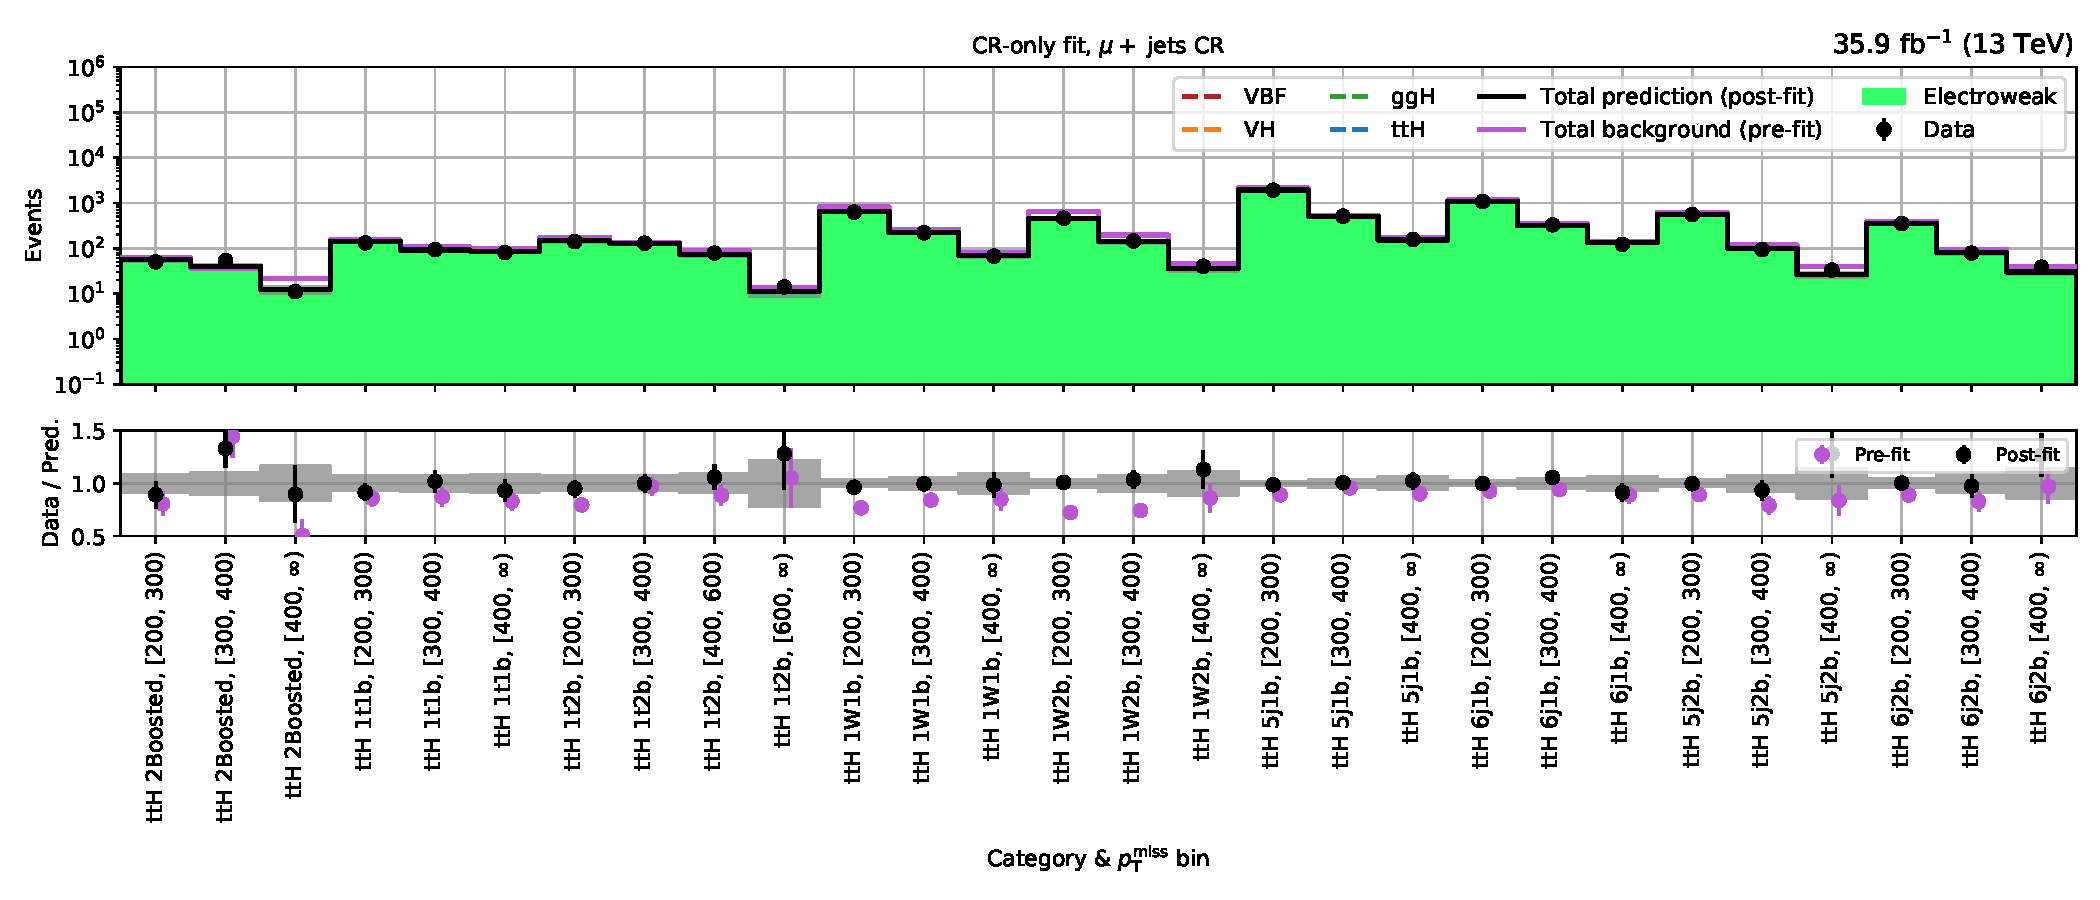
\includegraphics[width=\textwidth]{chapters/higgstoinv/figures/mountain_ranges/2016/ttH/Wmunu_tree_fit_b-abs_values_ttH_cats.pdf}
        \caption{\ttH --- \singleMuCr \gls{CR} (2016)}
    \end{subfigure}

    \begin{subfigure}[b]{\textwidth}
        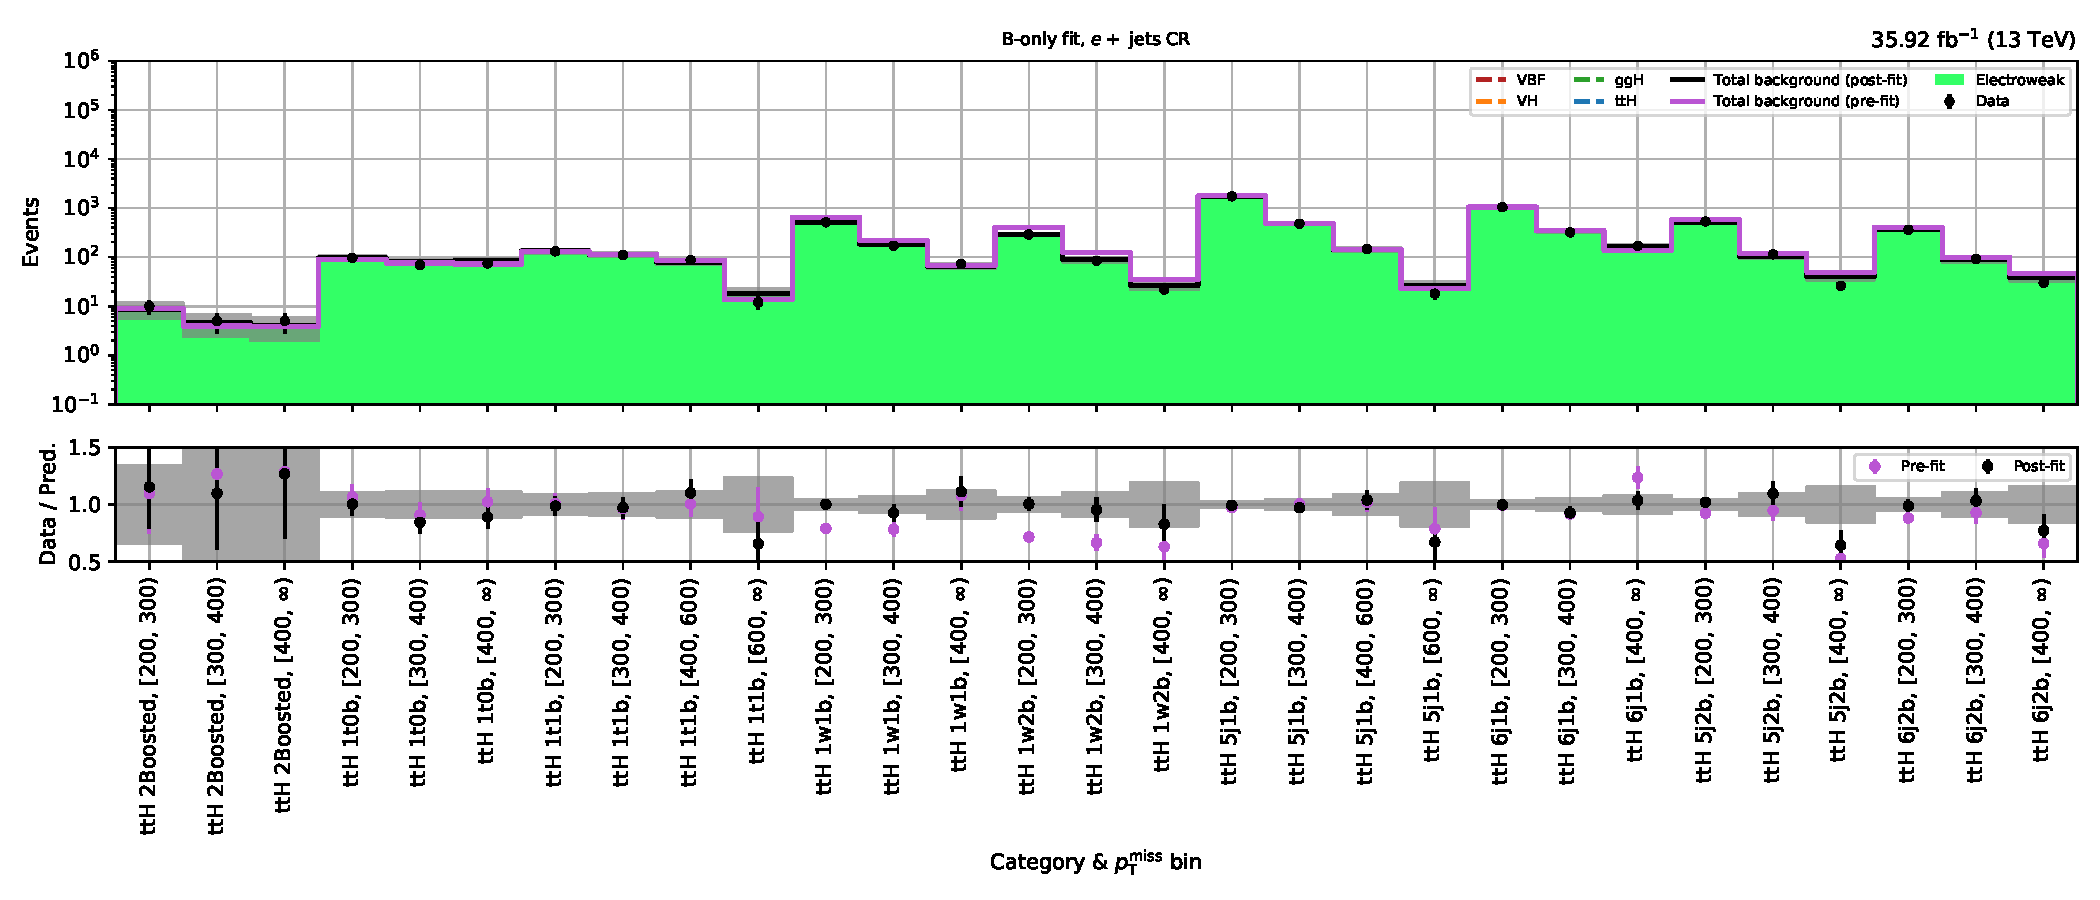
\includegraphics[width=\textwidth]{chapters/higgstoinv/figures/mountain_ranges/2016/ttH/Wenu_tree_fit_b-abs_values_ttH_cats.pdf}
        \caption{\ttH --- \singleEleCr \gls{CR} (2016)}
    \end{subfigure}
    \caption[Post-fit yields for each \ttH category and \ptmiss bin in the single lepton control regions for the 2016 dataset]{Post-fit yields for each \ttH category and \ptmiss bin in the single lepton \glspl{CR} for the 2016 dataset. The total background pre-fit and post-fit is compared to data in the lower panel of each subfigure.}
    \label{fig:htoinv_mountain_range_ttH_2016_single_lep_CRs}
\end{figure}

\begin{figure}[htbp]
    \centering
    \begin{subfigure}[b]{\textwidth}
        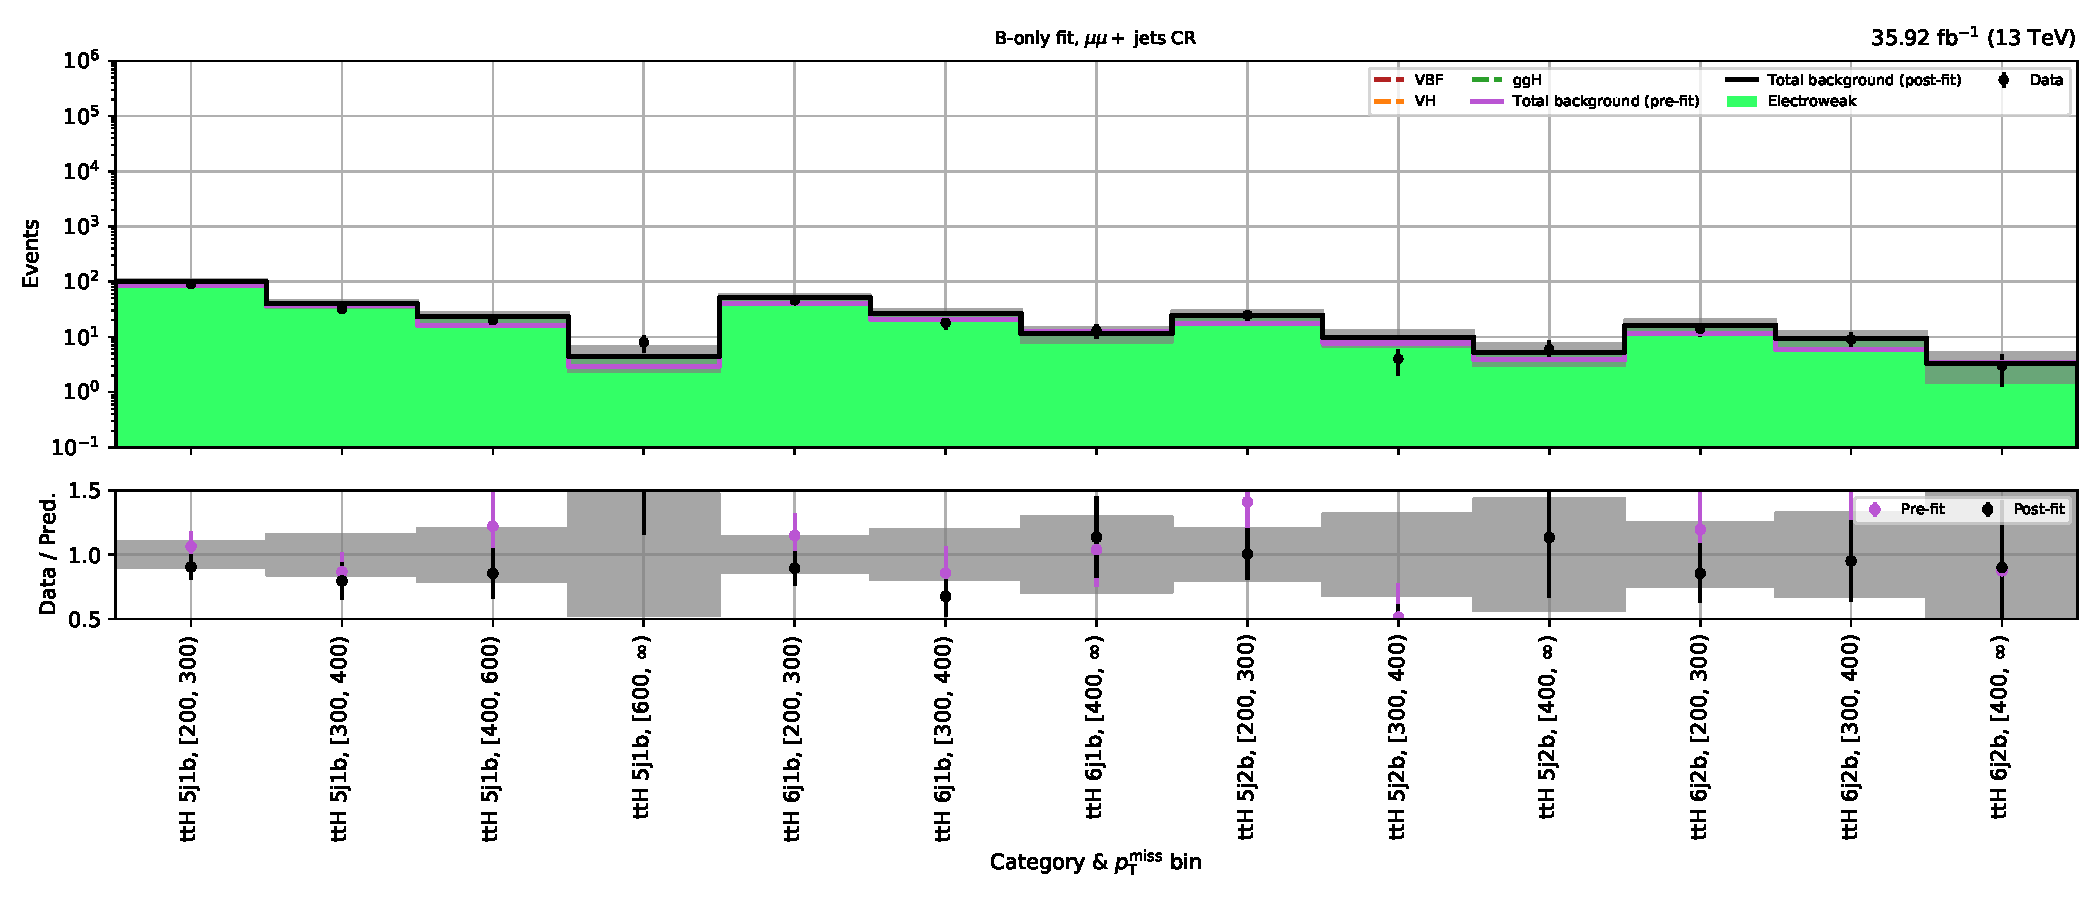
\includegraphics[width=\textwidth]{chapters/higgstoinv/figures/mountain_ranges/2016/ttH/Zmumu_tree_fit_b-abs_values_ttH_cats.pdf}
        \caption{\ttH --- \doubleMuCr \gls{CR} (2016)}
    \end{subfigure}

    \begin{subfigure}[b]{\textwidth}
        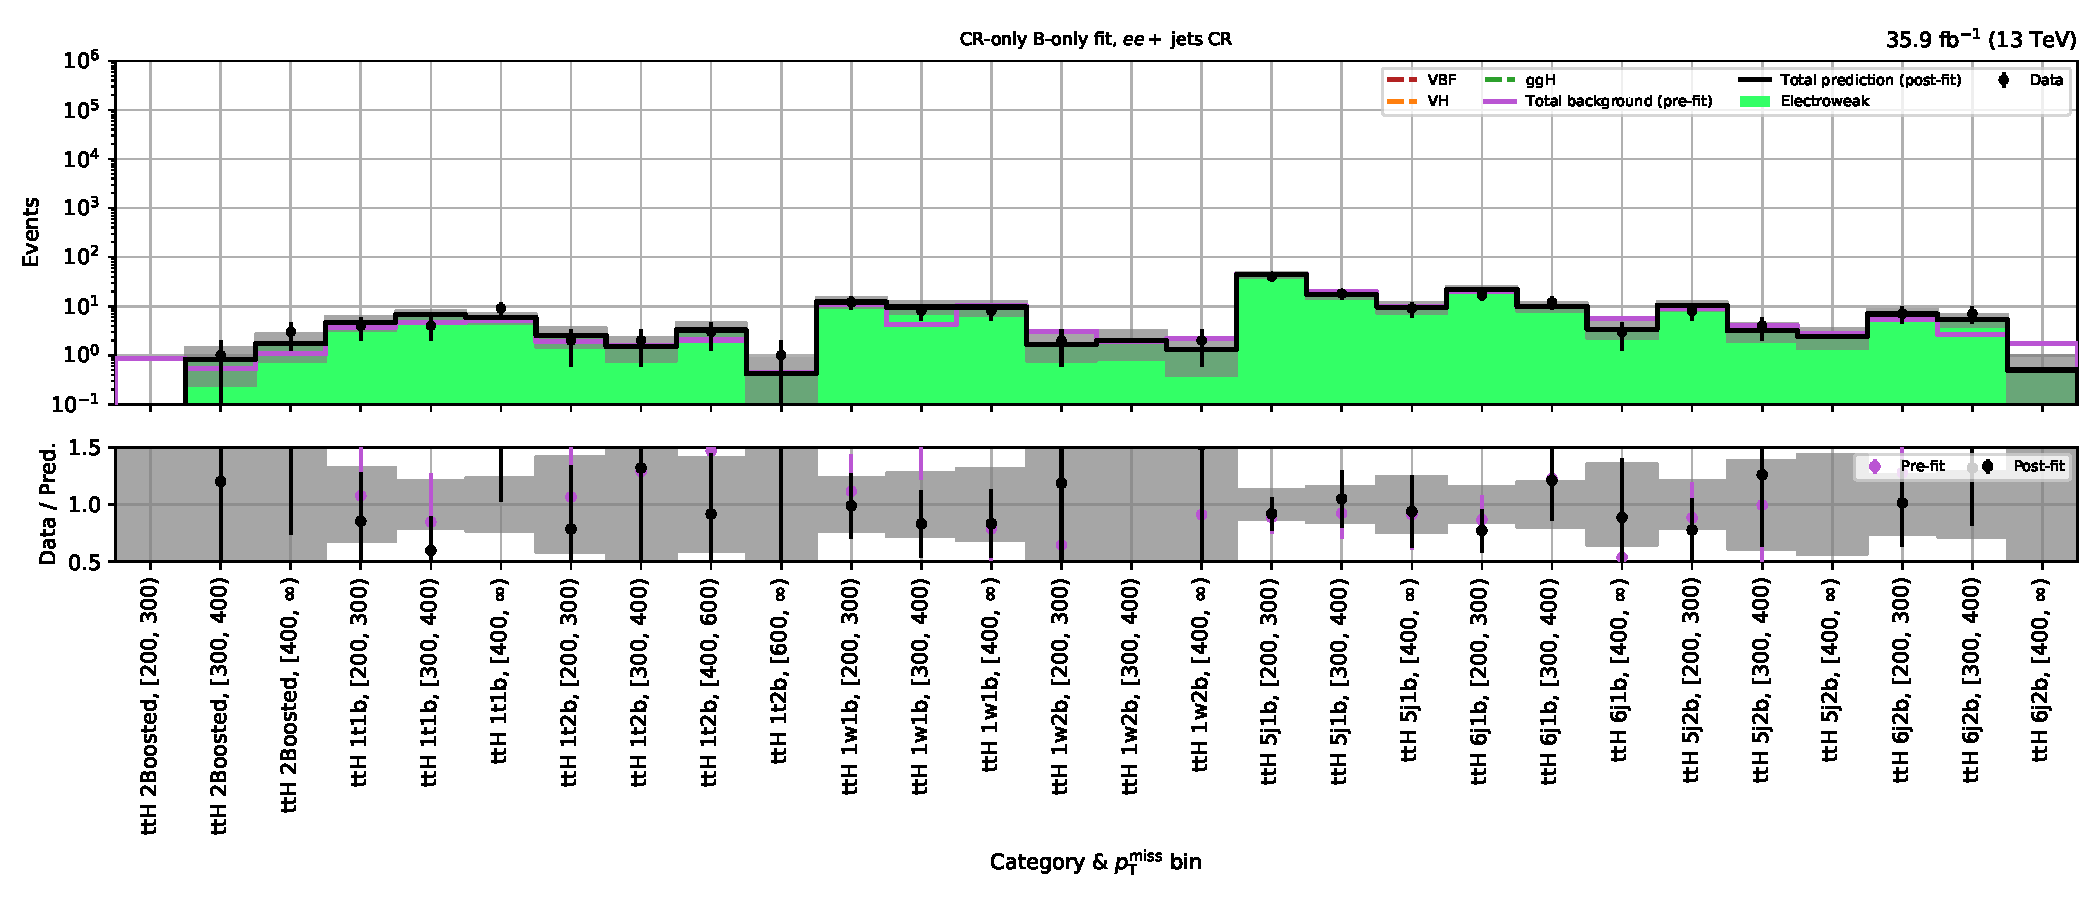
\includegraphics[width=\textwidth]{chapters/higgstoinv/figures/mountain_ranges/2016/ttH/Zee_tree_fit_b-abs_values_ttH_cats.pdf}
        \caption{\ttH --- \doubleEleCr \gls{CR} (2016)}
    \end{subfigure}
    \caption[Post-fit yields for each \ttH category and \ptmiss bin in the dilepton control regions for the 2016 dataset]{Post-fit yields for each \ttH category and \ptmiss bin in the dilepton \glspl{CR} for the 2016 dataset. The total background pre-fit and post-fit is compared to data in the lower panel of each subfigure.}
    \label{fig:htoinv_mountain_range_ttH_2016_dilep_CRs}
\end{figure}

\begin{figure}[htbp]
    \centering
    \begin{subfigure}[b]{\textwidth}
        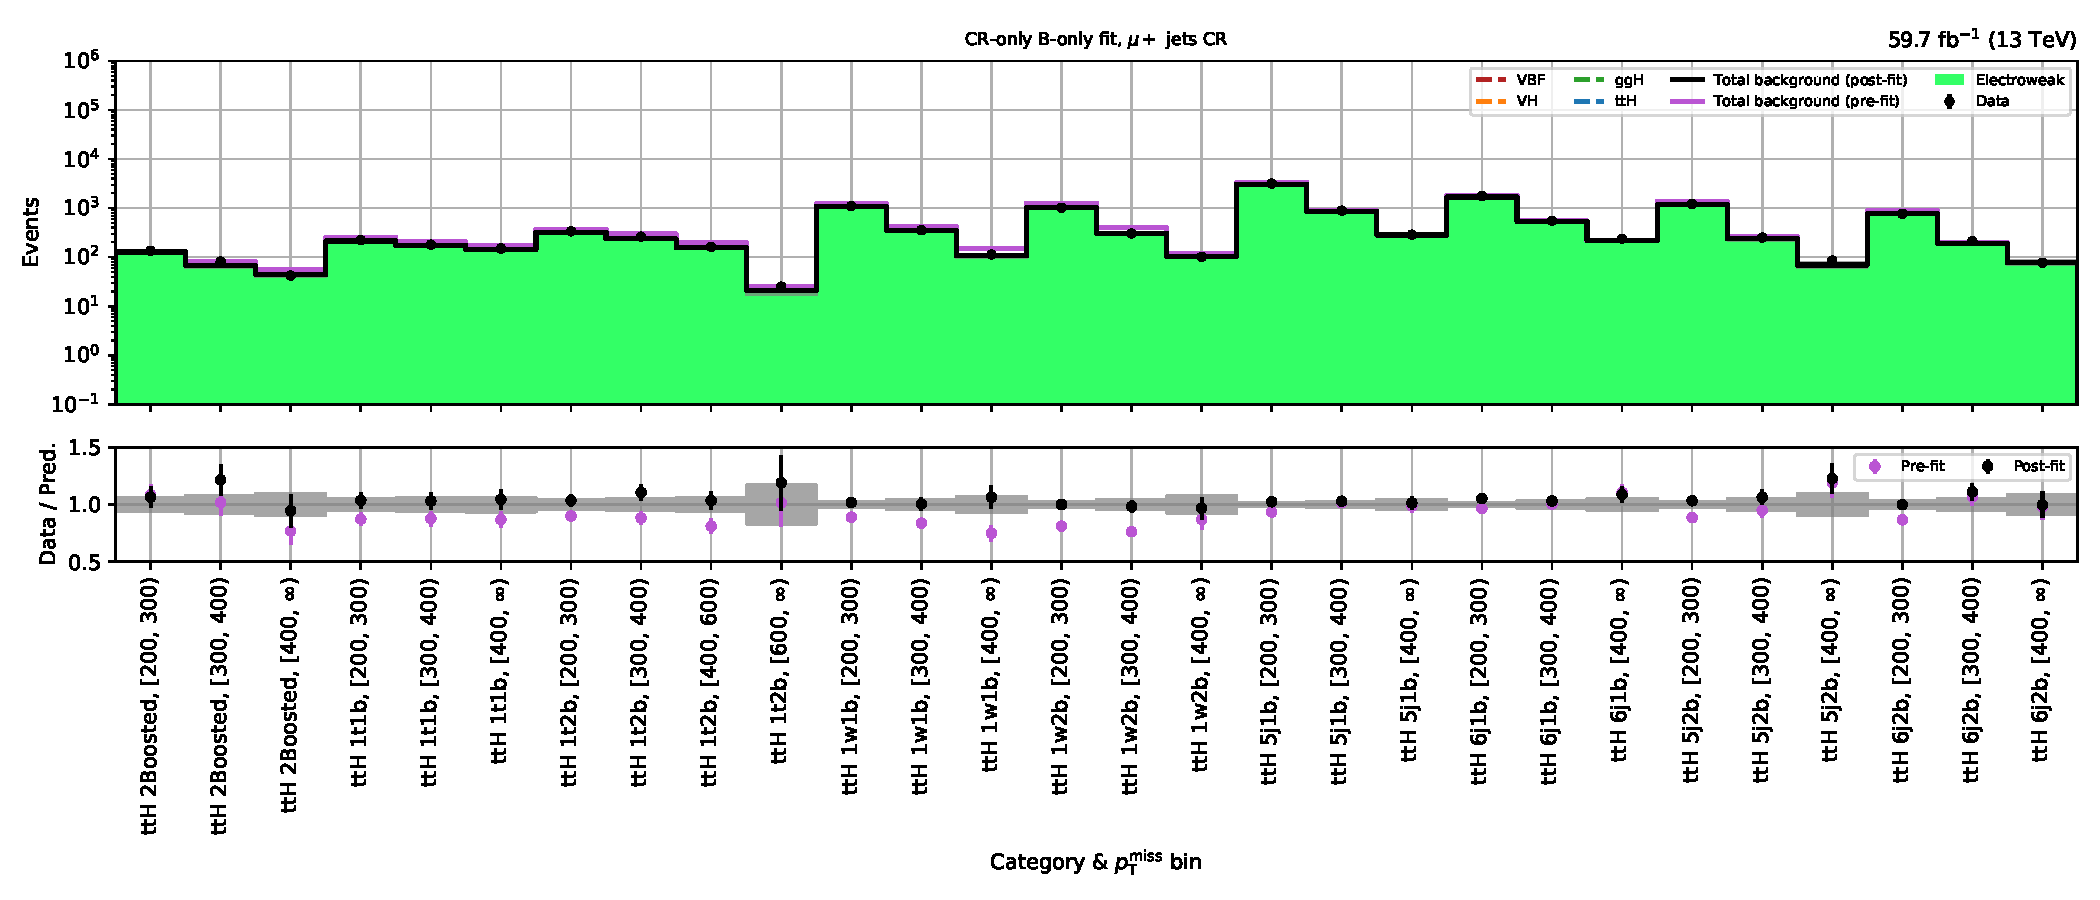
\includegraphics[width=\textwidth]{chapters/higgstoinv/figures/mountain_ranges/2018/ttH/Wmunu_tree_fit_b-abs_values_ttH_cats.pdf}
        \caption{\ttH --- \singleMuCr \gls{CR} (2018)}
    \end{subfigure}

    \begin{subfigure}[b]{\textwidth}
        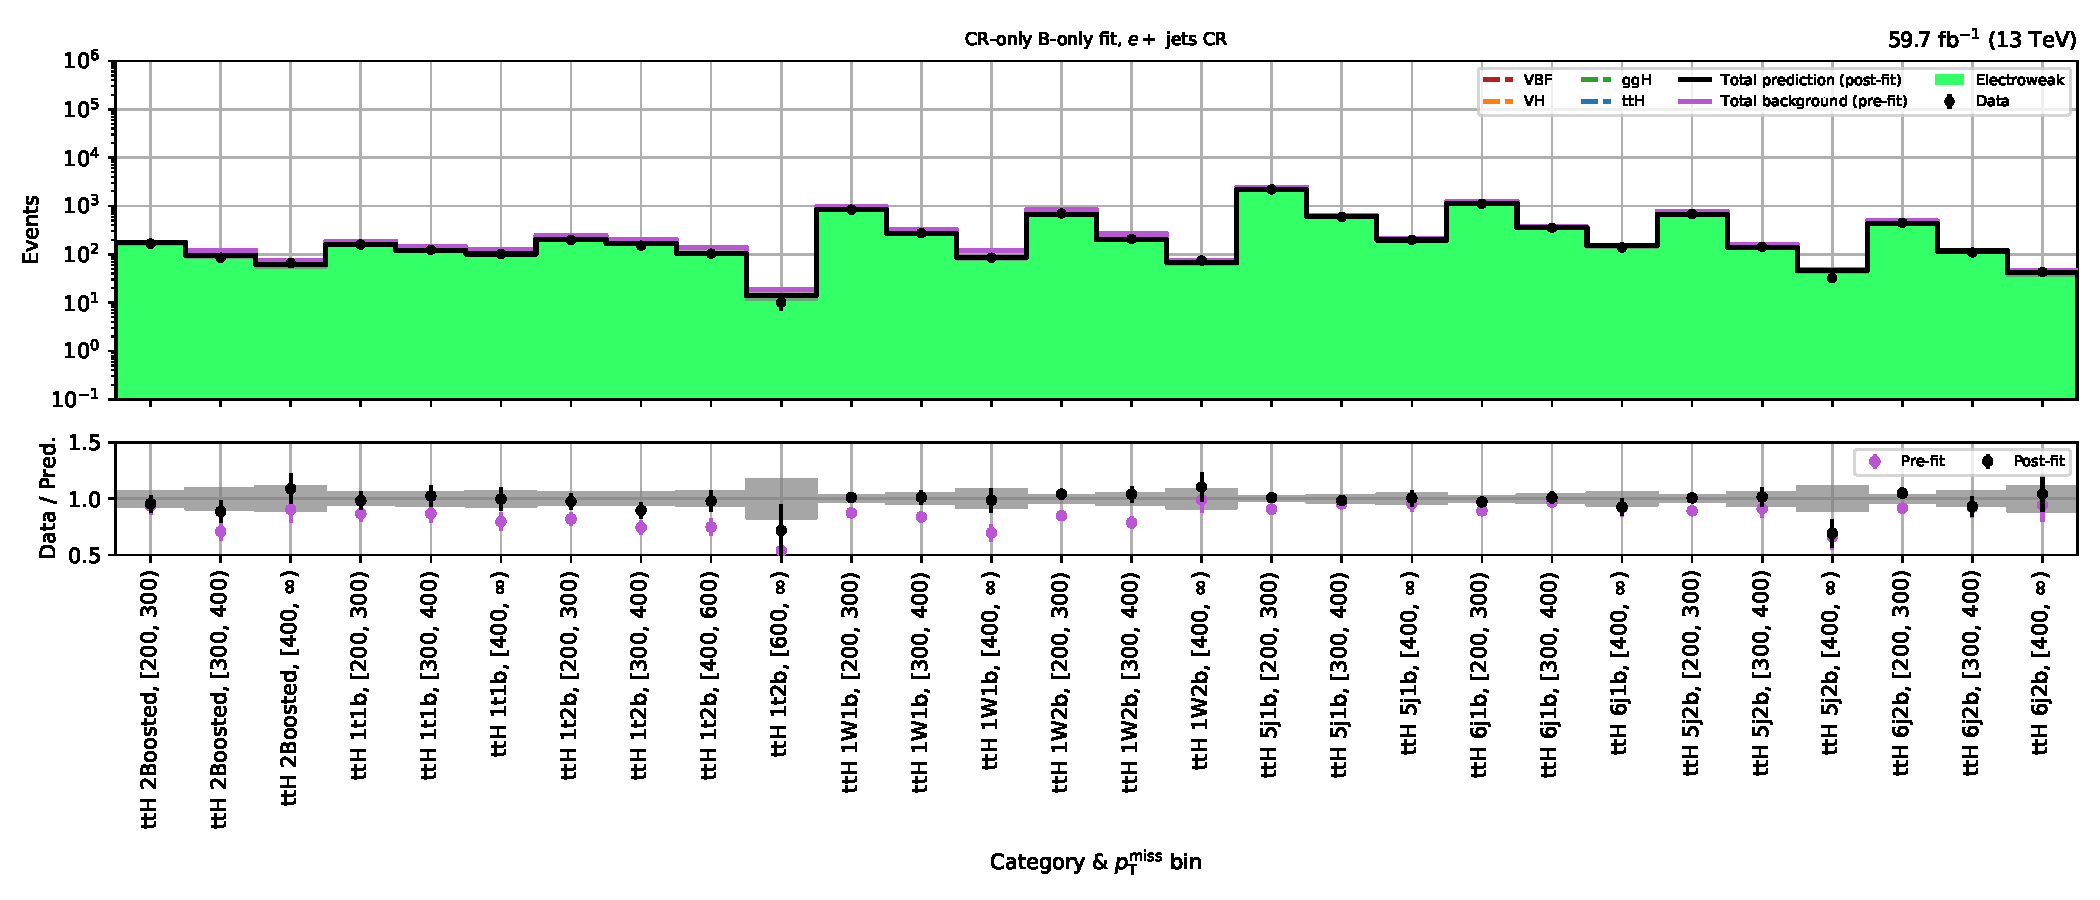
\includegraphics[width=\textwidth]{chapters/higgstoinv/figures/mountain_ranges/2018/ttH/Wenu_tree_fit_b-abs_values_ttH_cats.pdf}
        \caption{\ttH --- \singleEleCr \gls{CR} (2018)}
    \end{subfigure}
    \caption[Post-fit yields for each \ttH category and \ptmiss bin in the single lepton control regions for the 2018 dataset]{Post-fit yields for each \ttH category and \ptmiss bin in the single lepton \glspl{CR} for the 2018 dataset. The total background pre-fit and post-fit is compared to data in the lower panel of each subfigure.}
    \label{fig:htoinv_mountain_range_ttH_2018_single_lep_CRs}
\end{figure}

\begin{figure}[htbp]
    \centering
    \begin{subfigure}[b]{\textwidth}
        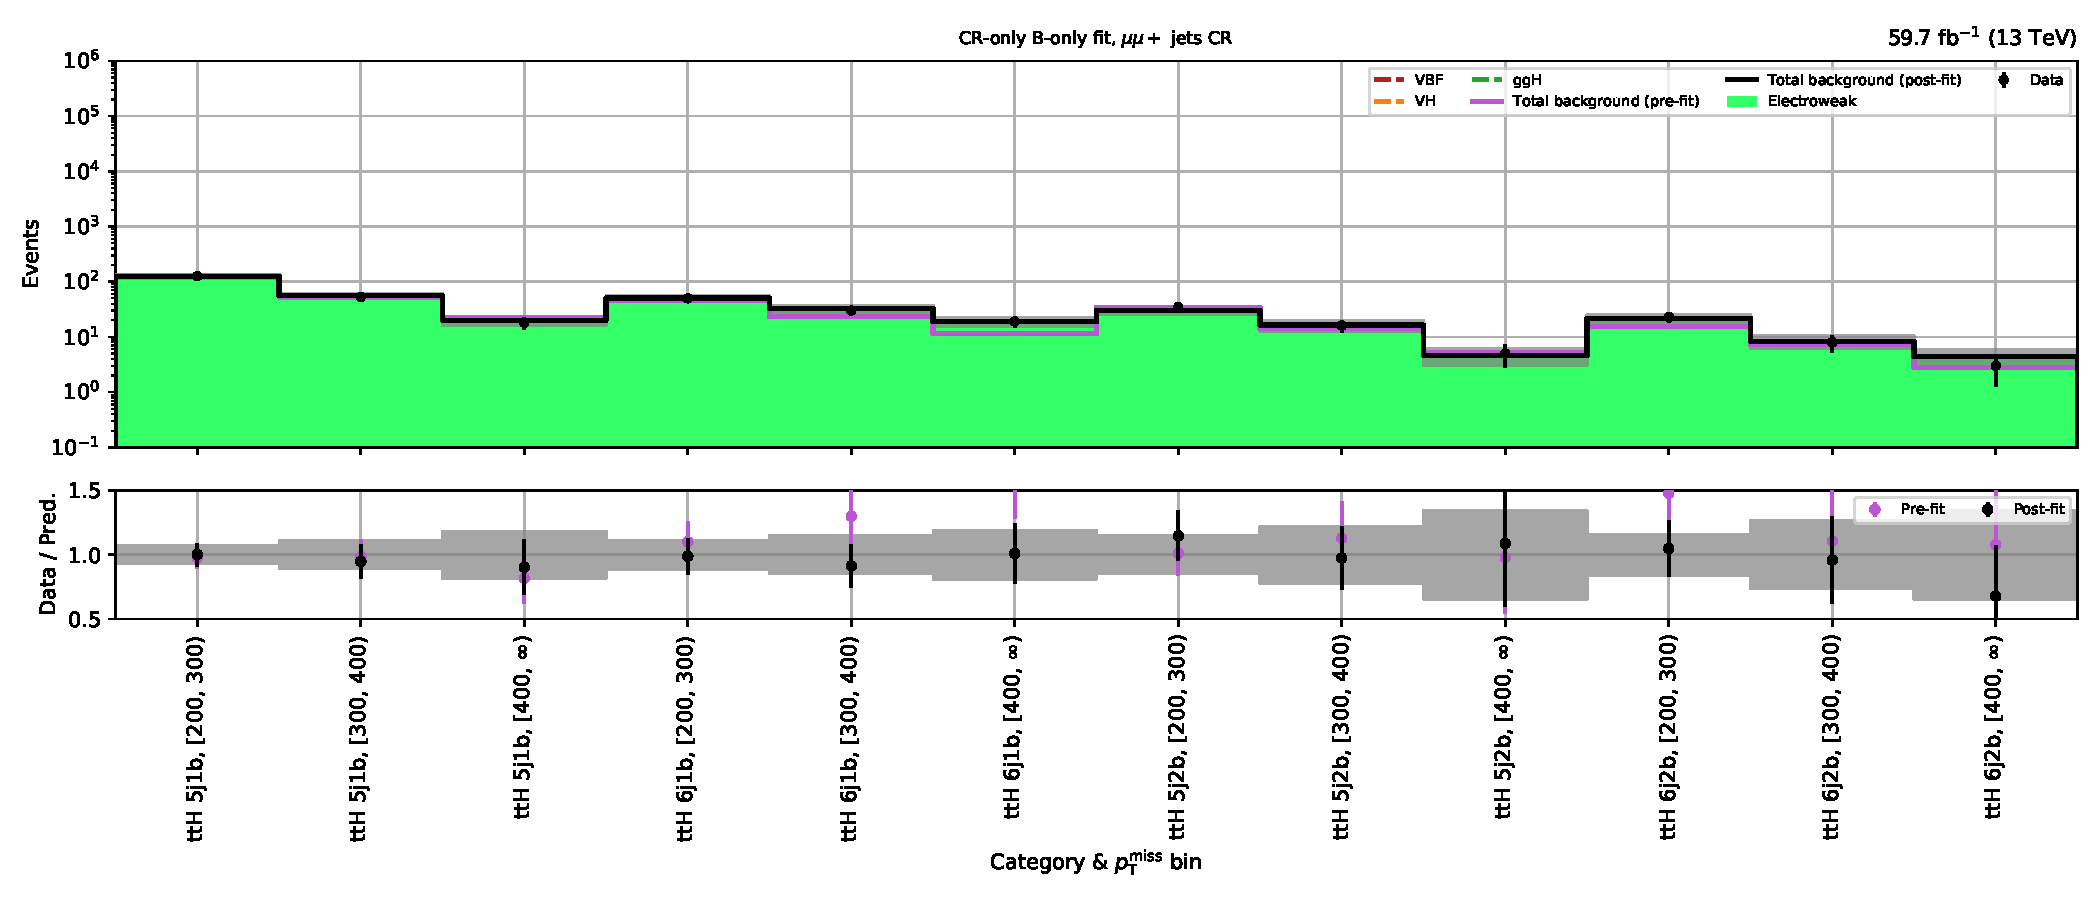
\includegraphics[width=\textwidth]{chapters/higgstoinv/figures/mountain_ranges/2018/ttH/Zmumu_tree_fit_b-abs_values_ttH_cats.pdf}
        \caption{\ttH --- \doubleMuCr \gls{CR} (2018)}
    \end{subfigure}

    \begin{subfigure}[b]{\textwidth}
        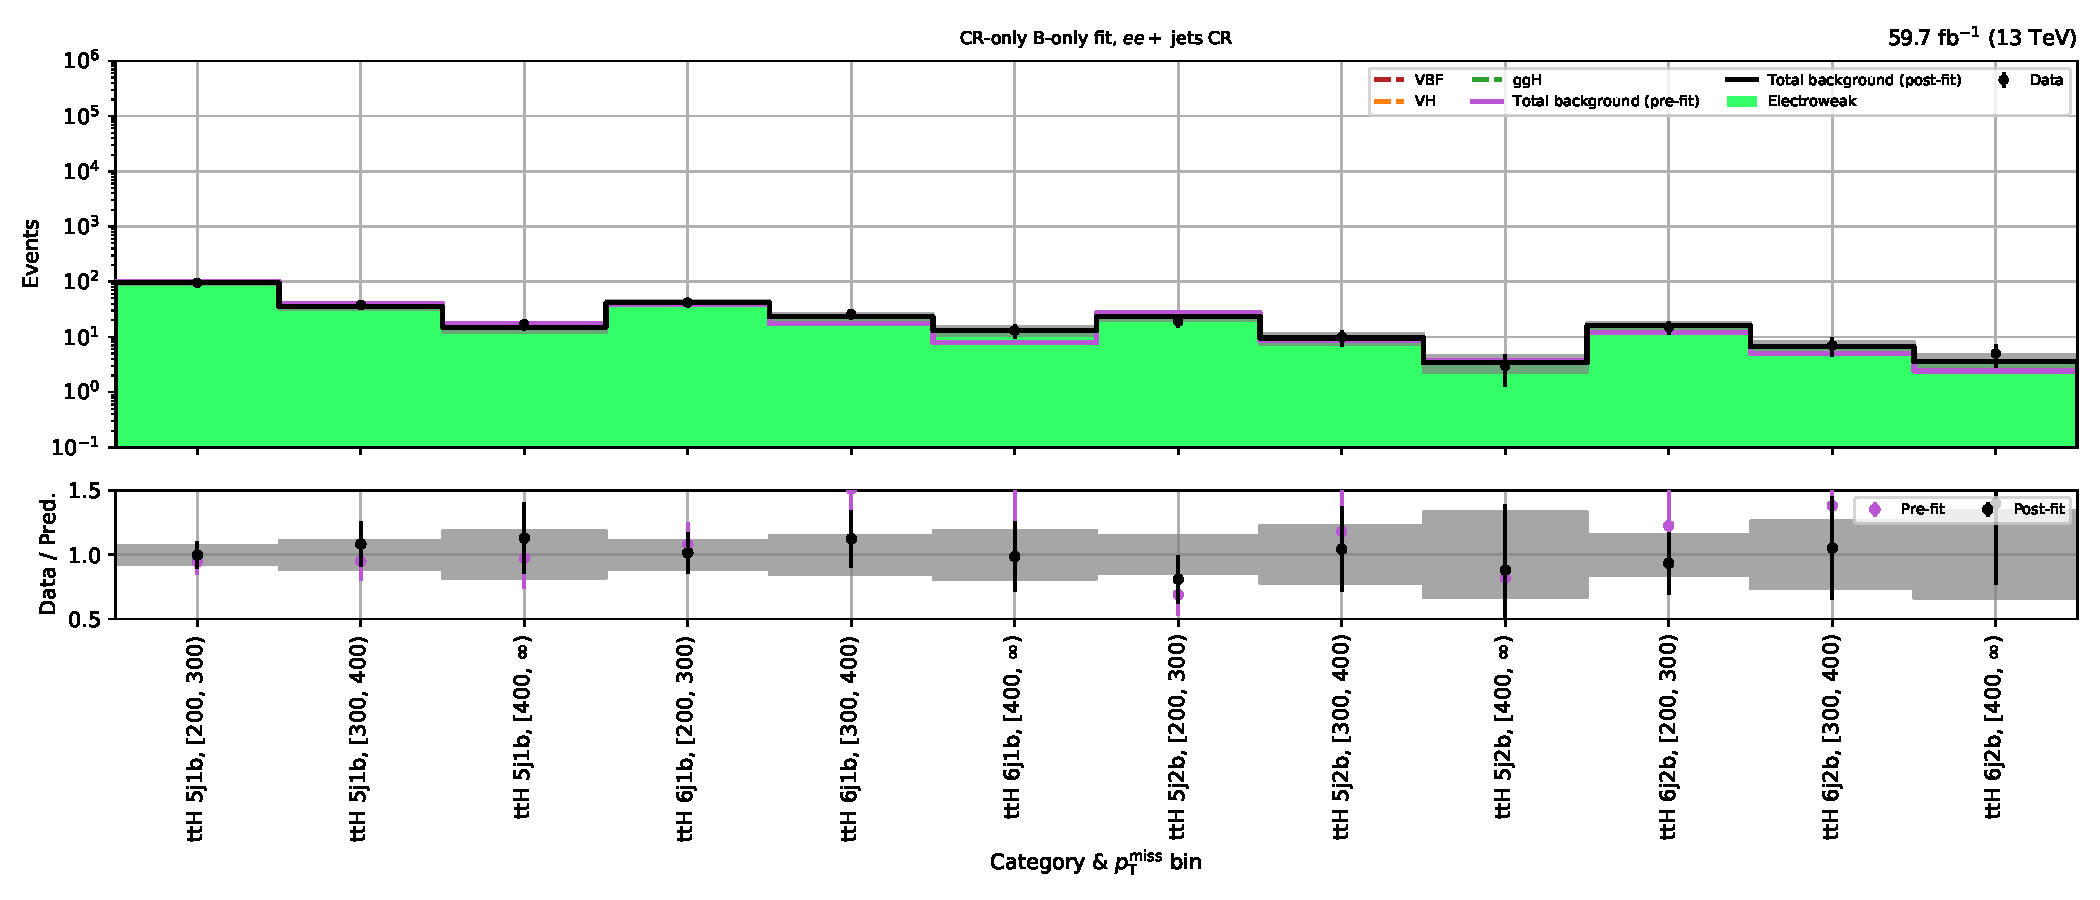
\includegraphics[width=\textwidth]{chapters/higgstoinv/figures/mountain_ranges/2018/ttH/Zee_tree_fit_b-abs_values_ttH_cats.pdf}
        \caption{\ttH --- \doubleEleCr \gls{CR} (2018)}
    \end{subfigure}
    \caption[Post-fit yields for each \ttH category and \ptmiss bin in the dilepton control regions for the 2018 dataset]{Post-fit yields for each \ttH category and \ptmiss bin in the dilepton \glspl{CR} for the 2018 dataset. The total background pre-fit and post-fit is compared to data in the lower panel of each subfigure.}
    \label{fig:htoinv_mountain_range_ttH_2018_dilep_CRs}
\end{figure}

\clearpage


%=========================================================


\section{Control region-only fits to the \texorpdfstring{\VH}{VH} categories}
\label{sec:pre_post_fit_plots_VH_CRs}

\begin{figure}[htbp]
    \centering
    \begin{subfigure}[b]{\textwidth}
        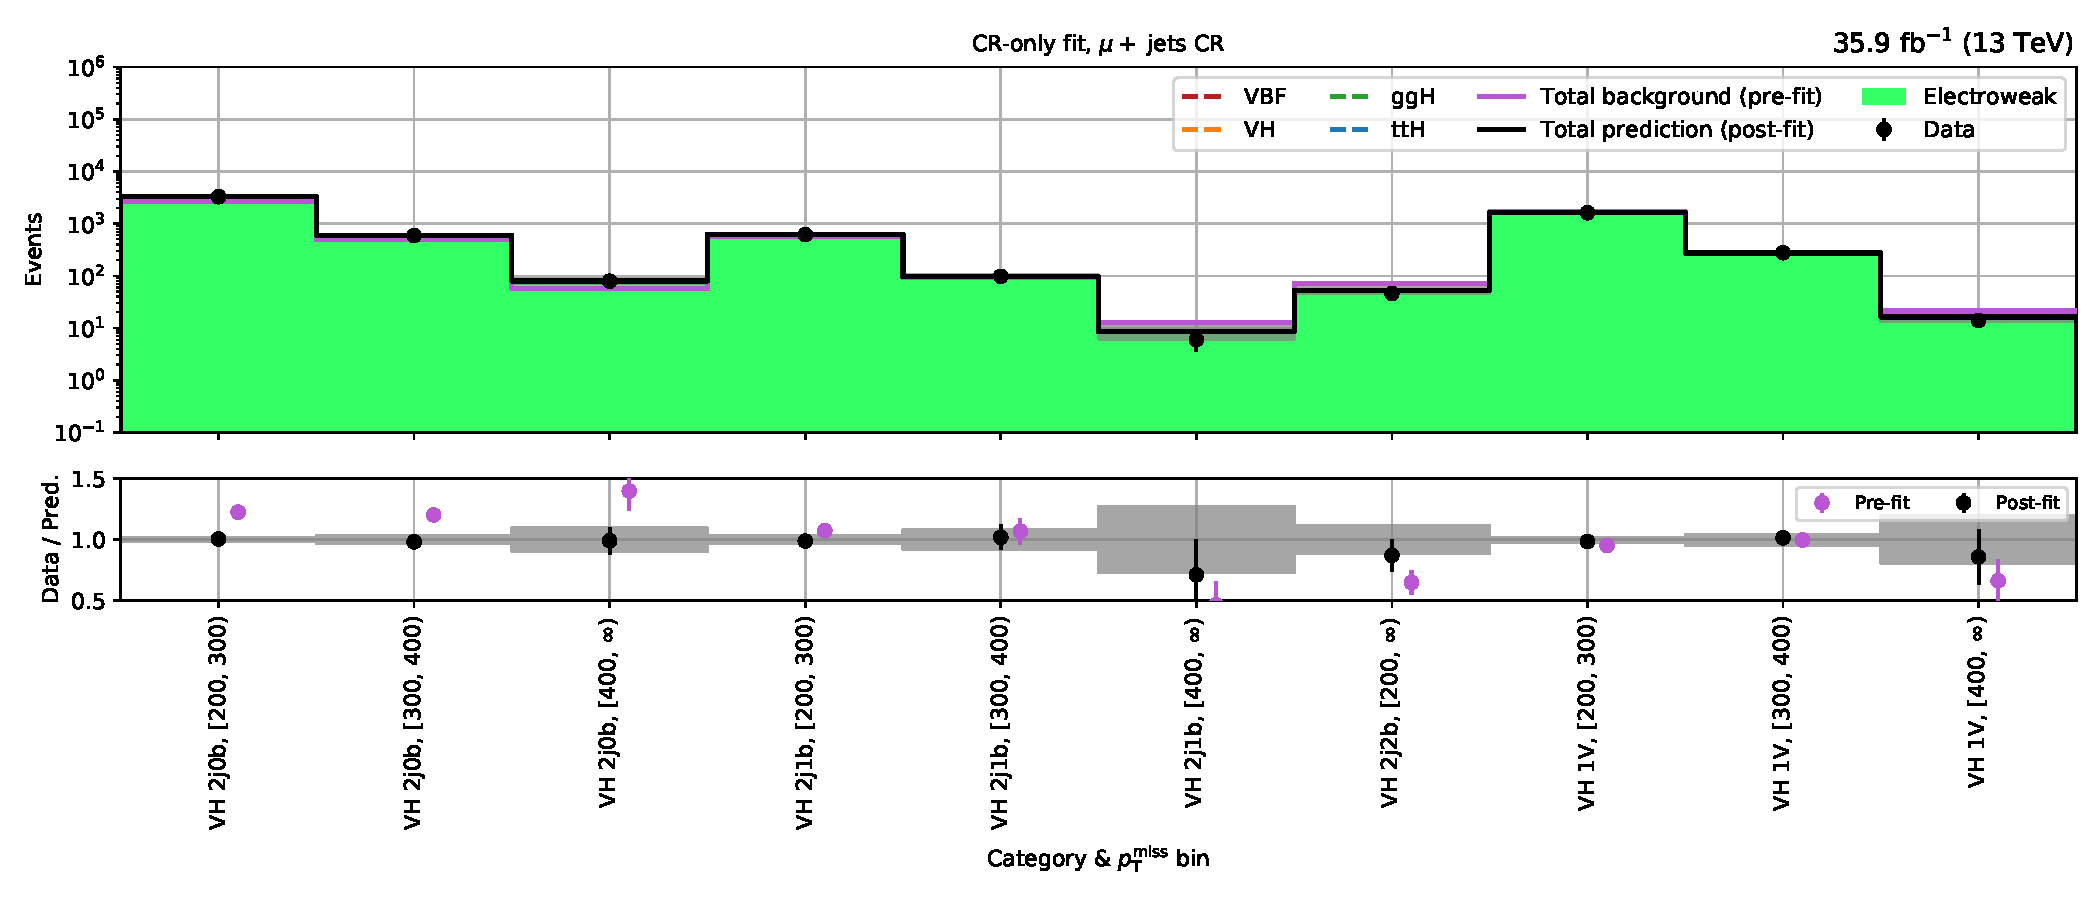
\includegraphics[width=\textwidth]{chapters/higgstoinv/figures/mountain_ranges/2016/VH/Wmunu_tree_fit_b-abs_values_VH_cats.pdf}
        \caption{\VH --- \singleMuCr \gls{CR} (2016)}
    \end{subfigure}

    \begin{subfigure}[b]{\textwidth}
        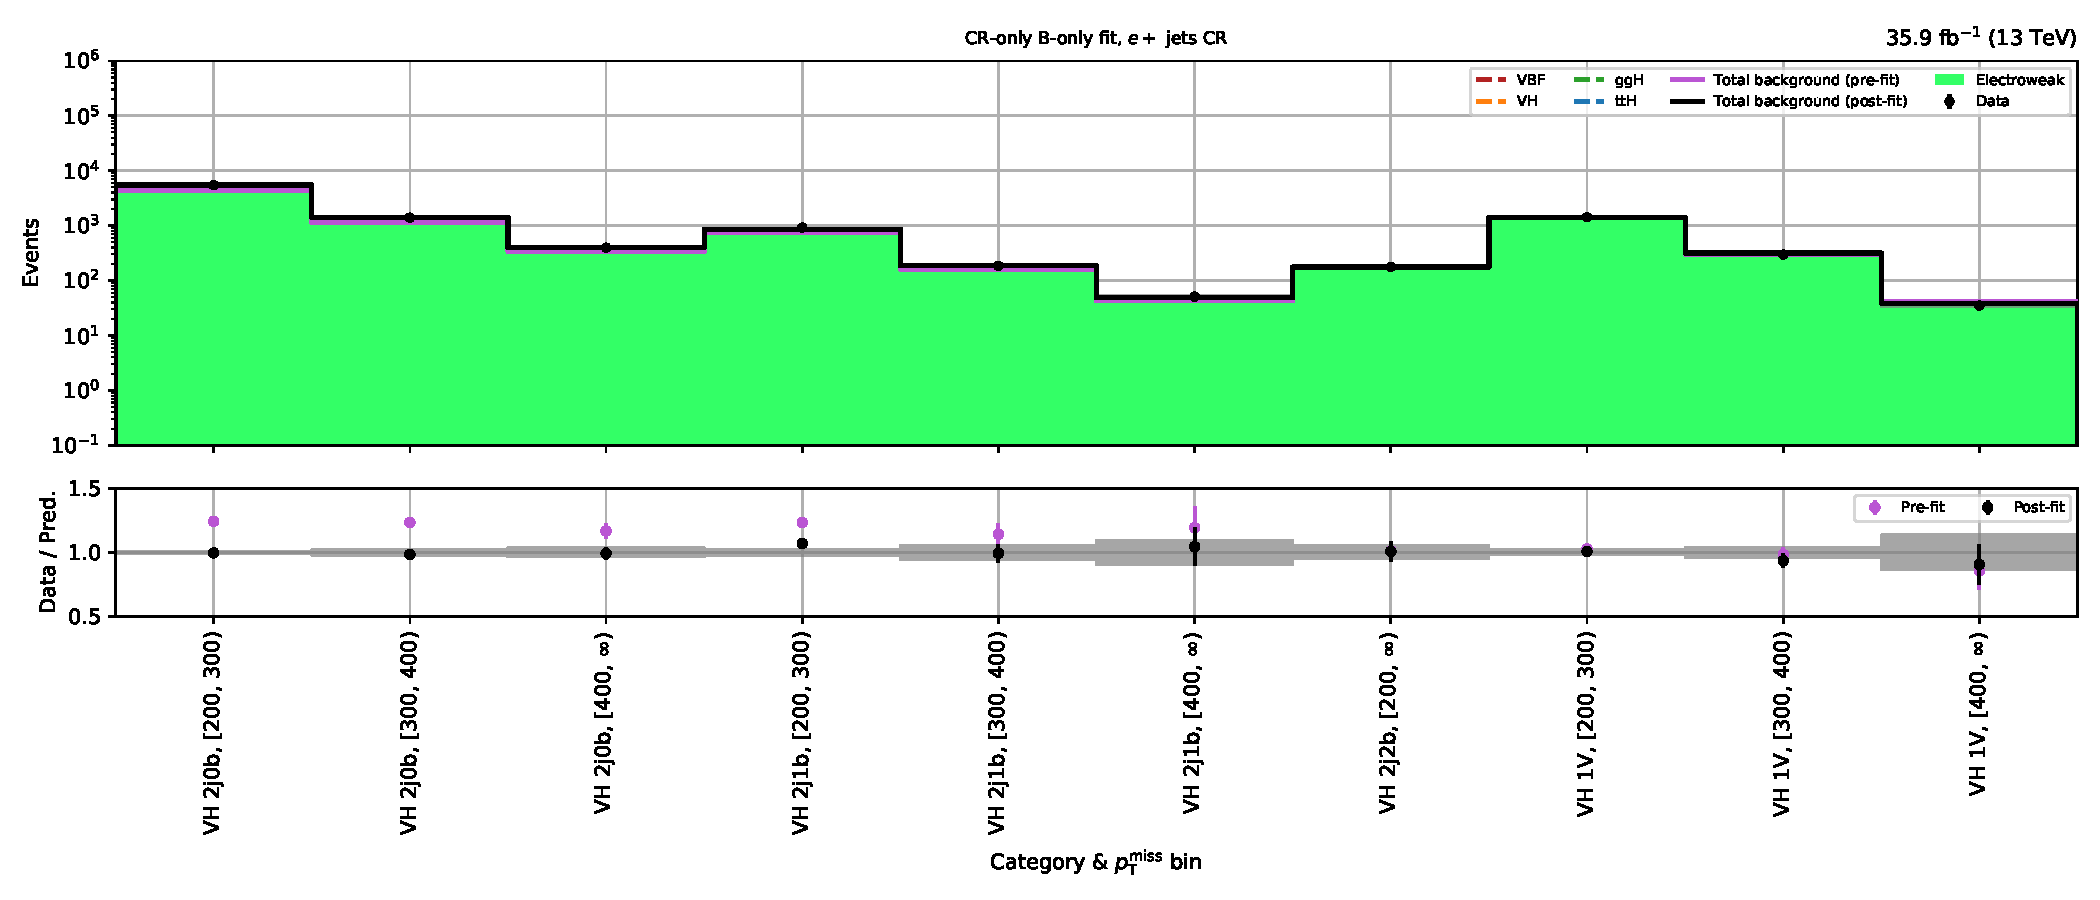
\includegraphics[width=\textwidth]{chapters/higgstoinv/figures/mountain_ranges/2016/VH/Wenu_tree_fit_b-abs_values_VH_cats.pdf}
        \caption{\VH --- \singleEleCr \gls{CR} (2016)}
    \end{subfigure}
    \caption[Post-fit yields for each \VH category and \ptmiss bin in the single lepton control regions for the 2016 dataset]{Post-fit yields for each \VH category and \ptmiss bin in the single lepton \glspl{CR} for the 2016 dataset. The total background pre-fit and post-fit is compared to data in the lower panel of each subfigure.}
    \label{fig:htoinv_mountain_range_VH_2016_single_lep_CRs}
\end{figure}

\begin{figure}[htbp]
    \centering
    \begin{subfigure}[b]{0.9\textwidth}
        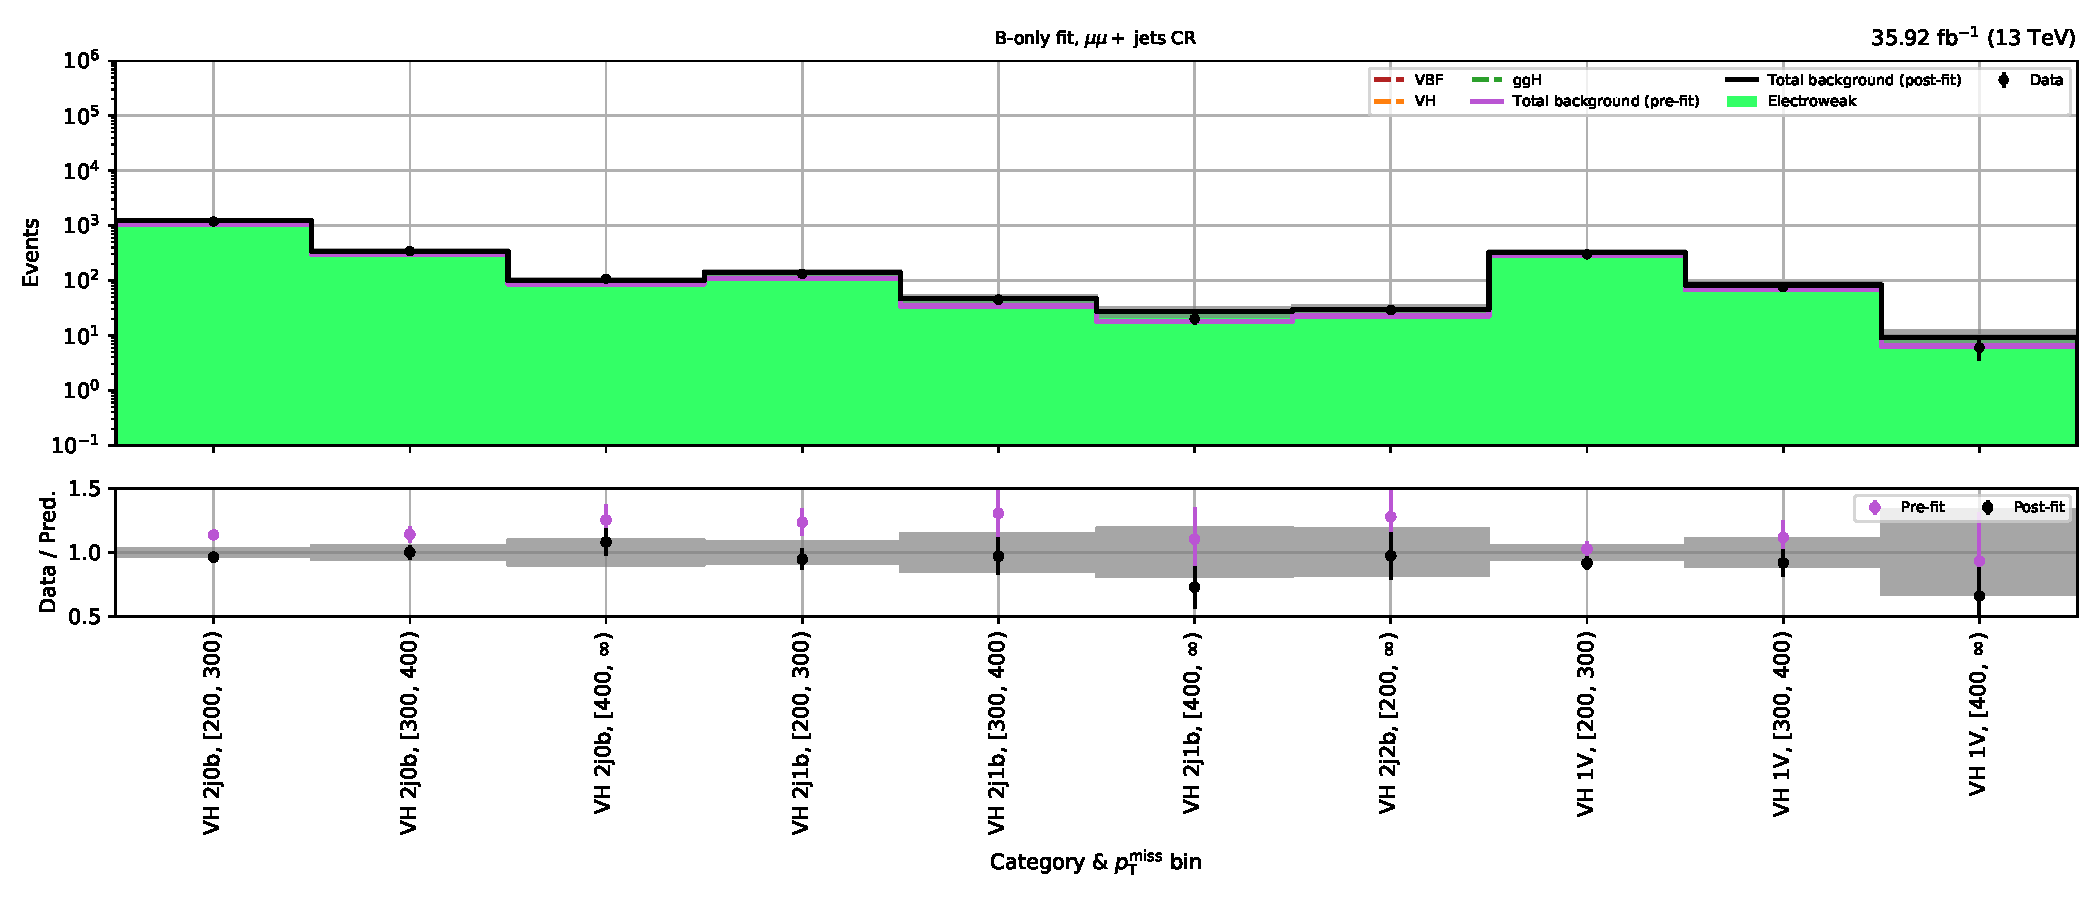
\includegraphics[width=\textwidth]{chapters/higgstoinv/figures/mountain_ranges/2016/VH/Zmumu_tree_fit_b-abs_values_VH_cats.pdf}
        \caption{\VH --- \doubleMuCr \gls{CR} (2016)}
    \end{subfigure}

    \begin{subfigure}[b]{0.9\textwidth}
        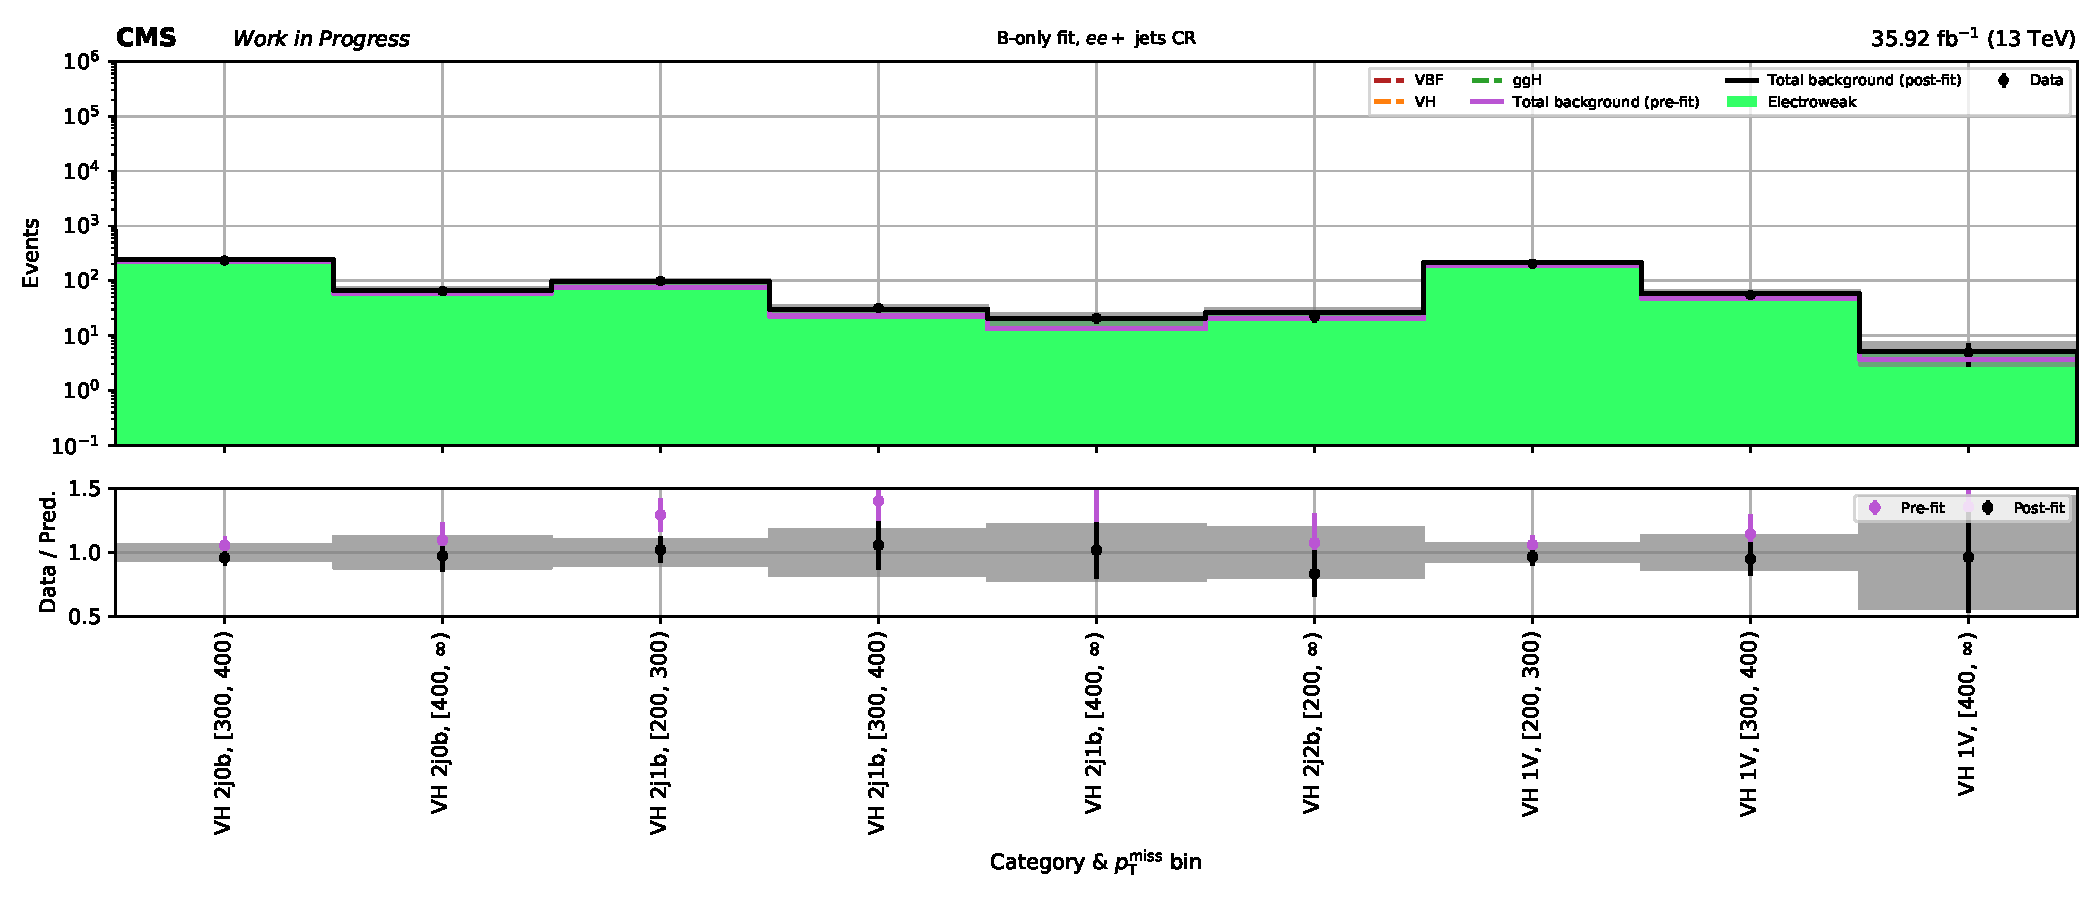
\includegraphics[width=\textwidth]{chapters/higgstoinv/figures/mountain_ranges/2016/VH/Zee_tree_fit_b-abs_values_VH_cats.pdf}
        \caption{\VH --- \doubleEleCr \gls{CR} (2016)}
    \end{subfigure}

    \begin{subfigure}[b]{0.9\textwidth}
        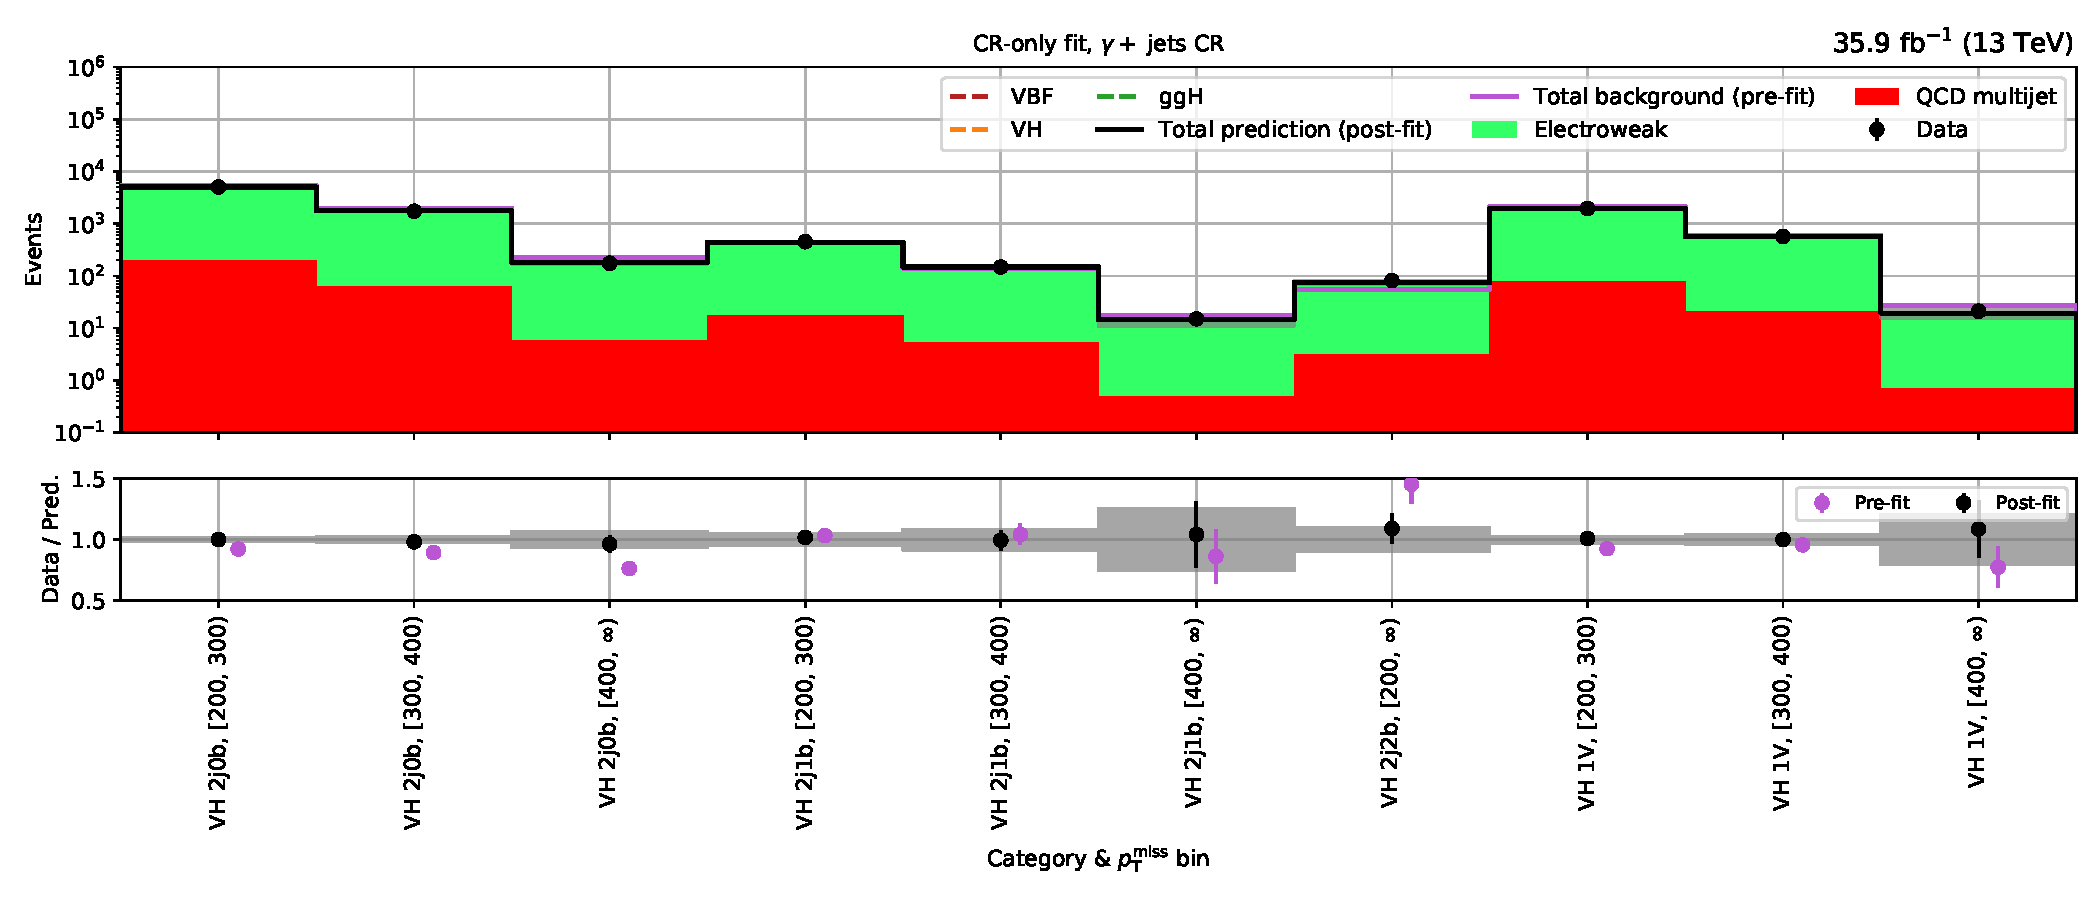
\includegraphics[width=\textwidth]{chapters/higgstoinv/figures/mountain_ranges/2016/VH/Photon_tree_fit_b-abs_values_VH_cats.pdf}
        \caption{\VH --- \singlePhotonCr \gls{CR} (2016)}
    \end{subfigure}
    \caption[Post-fit yields for each \VH category and \ptmiss bin in the dilepton and photon control regions for the 2016 dataset]{Post-fit yields for each \VH category and \ptmiss bin in the dilepton and photon \glspl{CR} for the 2016 dataset. The total background pre-fit and post-fit is compared to data in the lower panel of each subfigure.}
    \label{fig:htoinv_mountain_range_VH_2016_dilep_photon_CRs}
\end{figure}

\begin{figure}[htbp]
    \centering
    \begin{subfigure}[b]{\textwidth}
        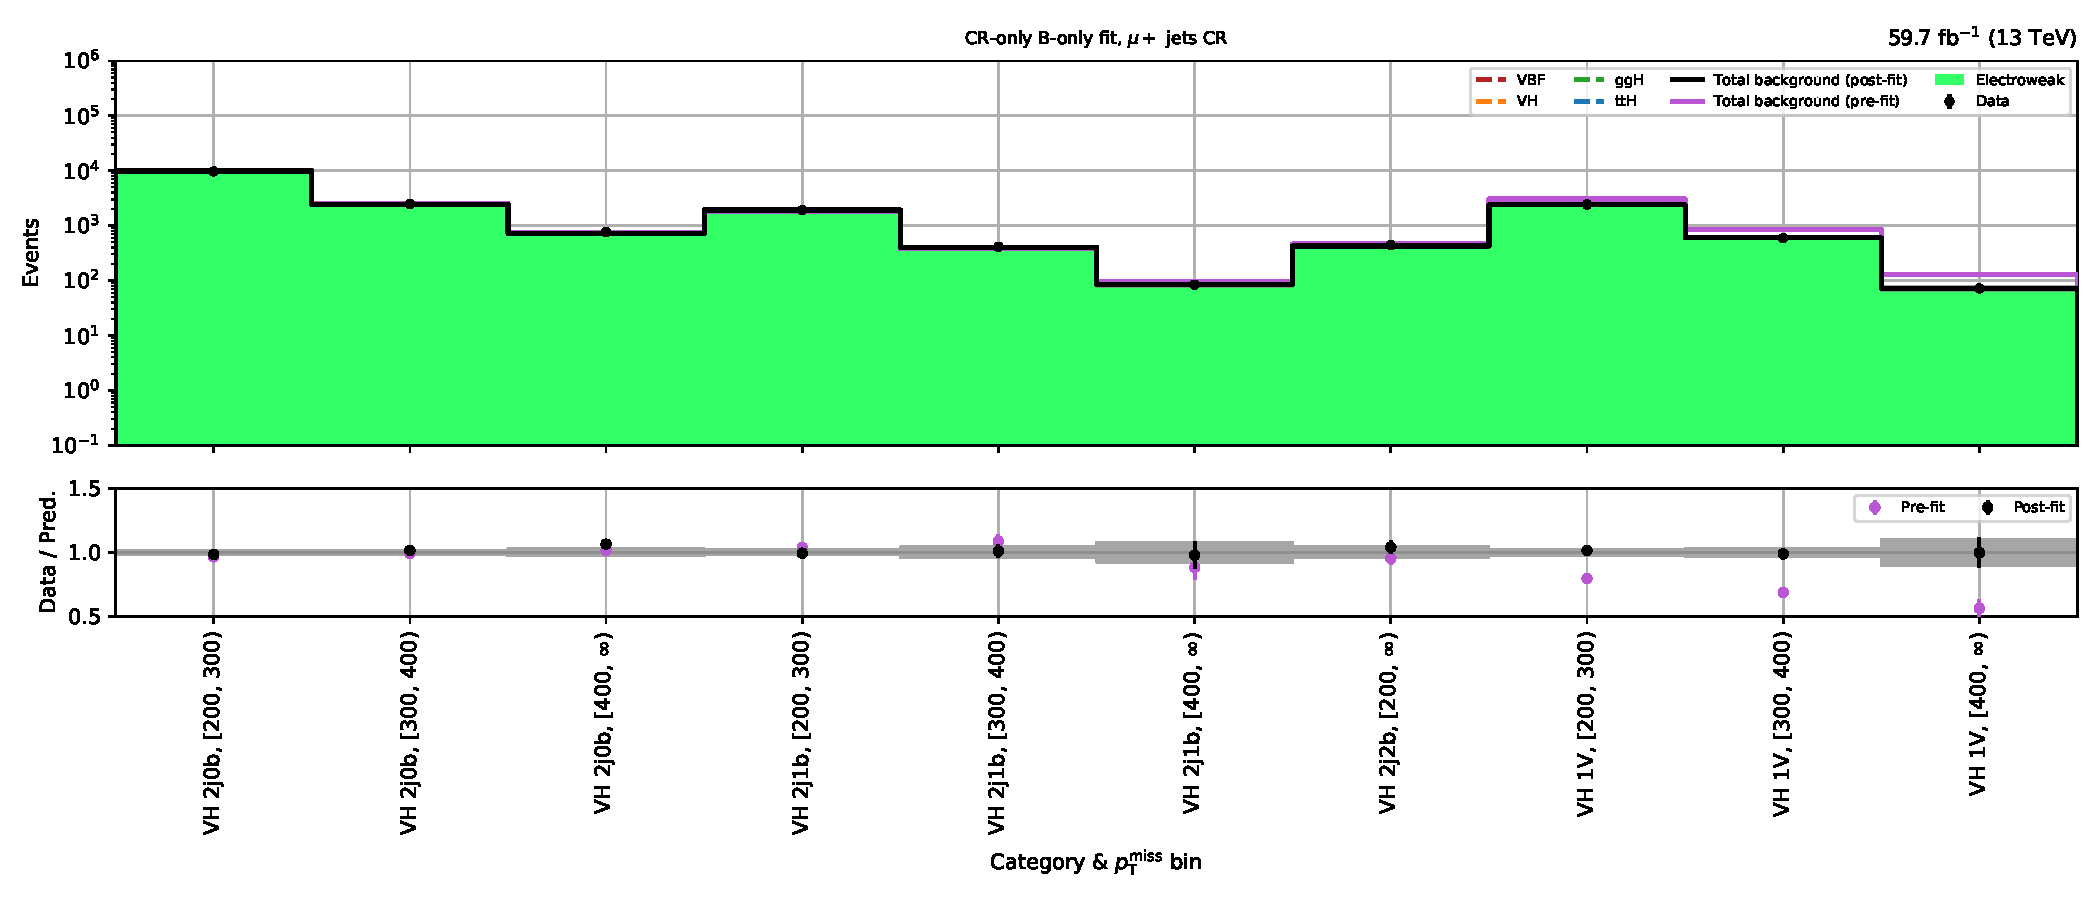
\includegraphics[width=\textwidth]{chapters/higgstoinv/figures/mountain_ranges/2018/VH/Wmunu_tree_fit_b-abs_values_VH_cats.pdf}
        \caption{\VH --- \singleMuCr \gls{CR} (2018)}
    \end{subfigure}

    \begin{subfigure}[b]{\textwidth}
        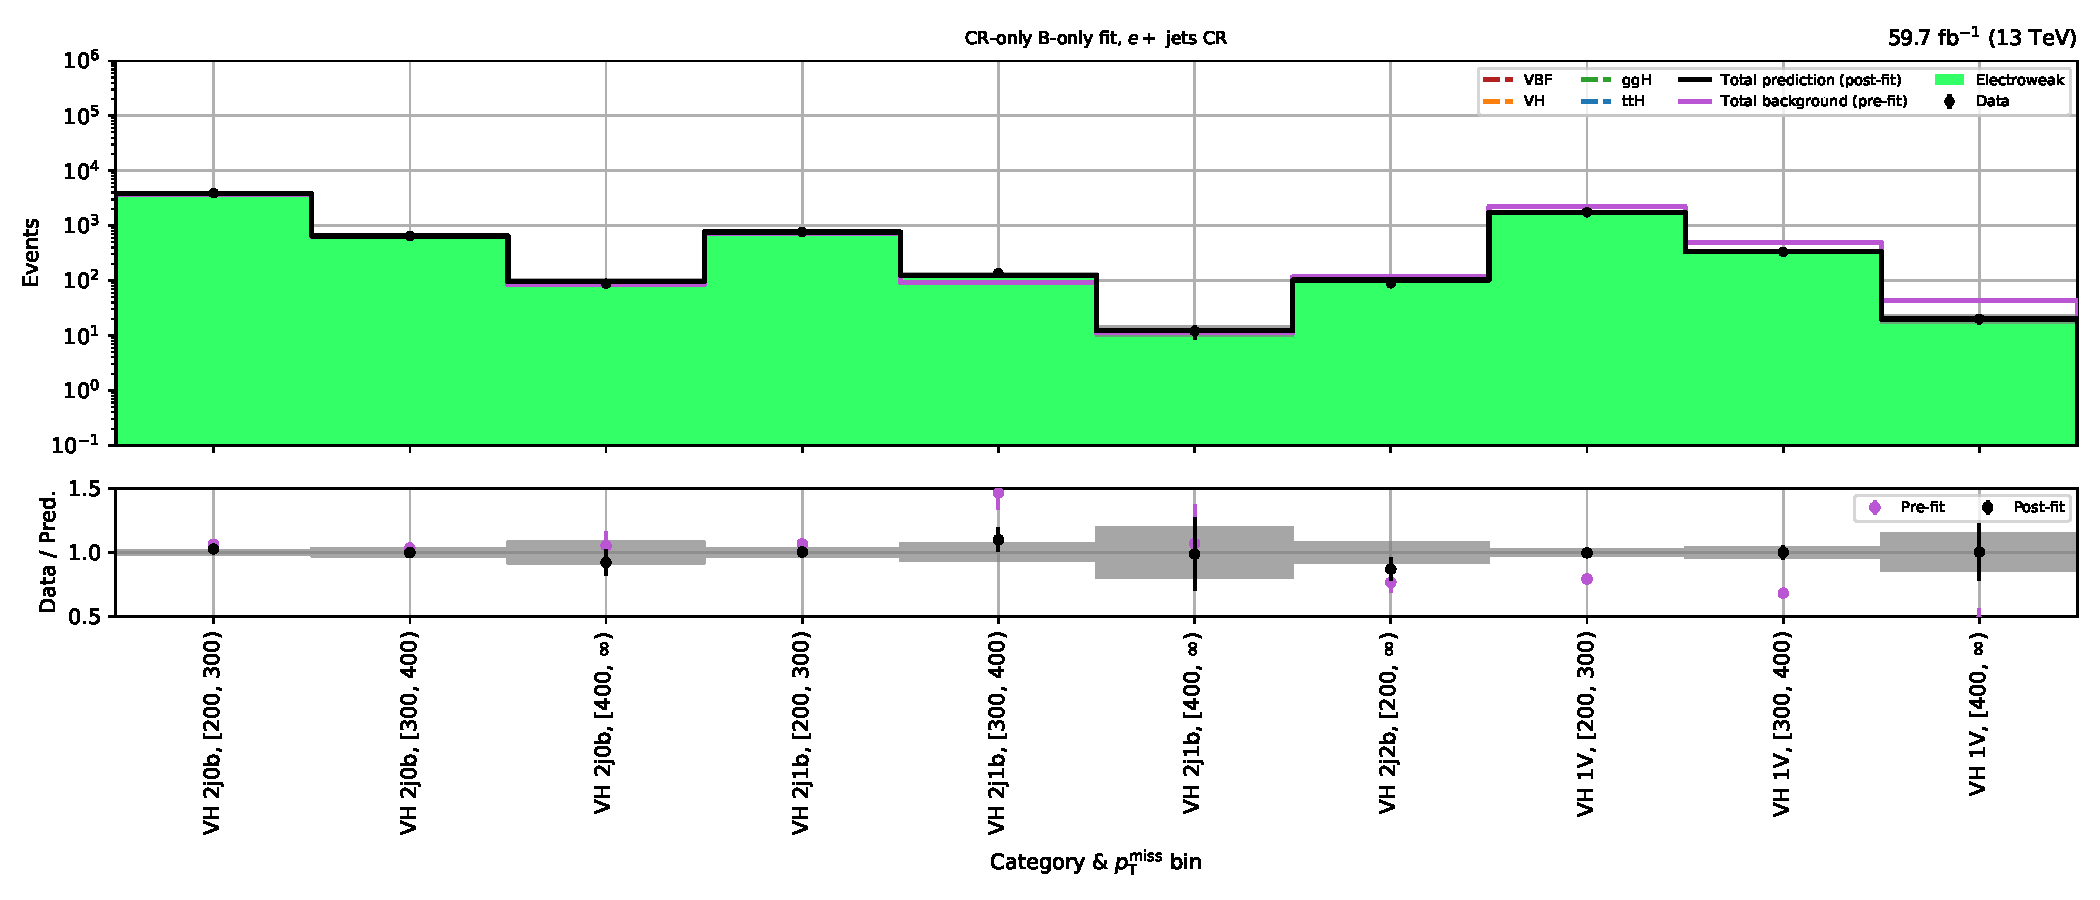
\includegraphics[width=\textwidth]{chapters/higgstoinv/figures/mountain_ranges/2018/VH/Wenu_tree_fit_b-abs_values_VH_cats.pdf}
        \caption{\VH --- \singleEleCr \gls{CR} (2018)}
    \end{subfigure}
    \caption[Post-fit yields for each \VH category and \ptmiss bin in the single lepton control regions for the 2018 dataset]{Post-fit yields for each \VH category and \ptmiss bin in the single lepton \glspl{CR} for the 2018 dataset. The total background pre-fit and post-fit is compared to data in the lower panel of each subfigure.}
    \label{fig:htoinv_mountain_range_VH_2018_single_lep_CRs}
\end{figure}

\begin{figure}[htbp]
    \centering
    \begin{subfigure}[b]{0.9\textwidth}
        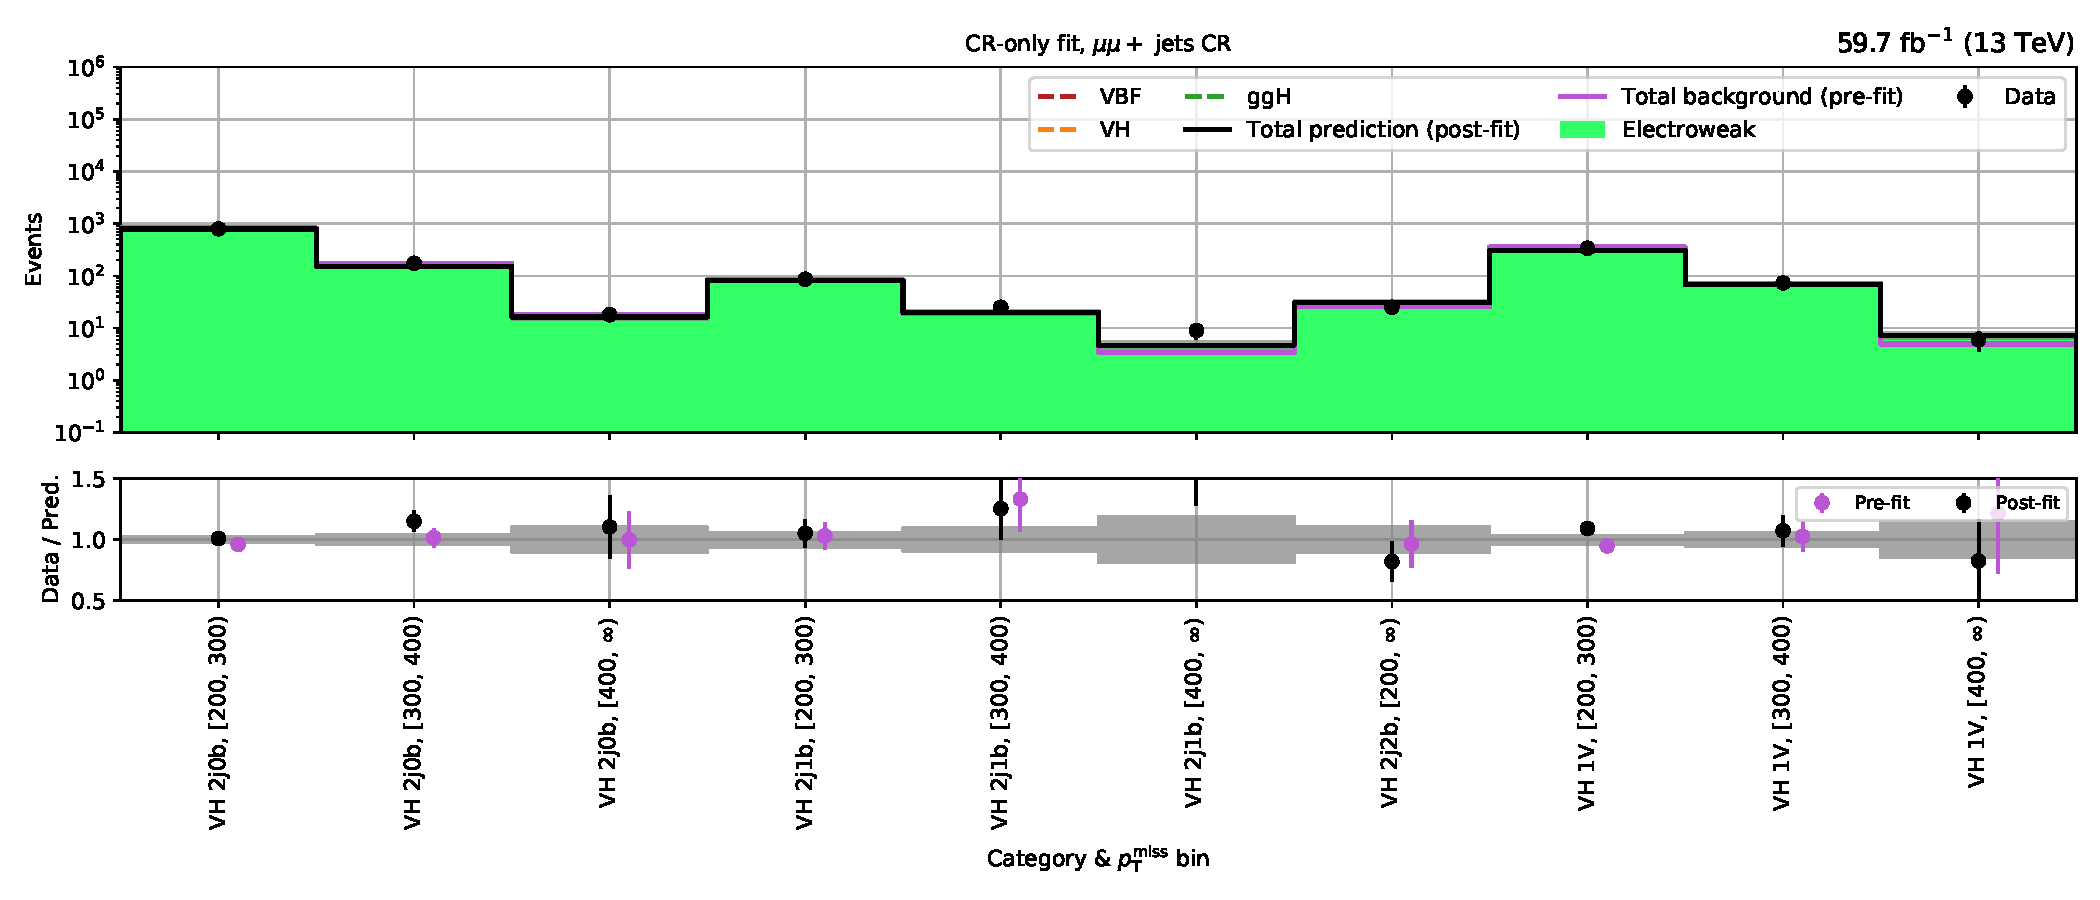
\includegraphics[width=\textwidth]{chapters/higgstoinv/figures/mountain_ranges/2018/VH/Zmumu_tree_fit_b-abs_values_VH_cats.pdf}
        \caption{\VH --- \doubleMuCr \gls{CR} (2018)}
    \end{subfigure}

    \begin{subfigure}[b]{0.9\textwidth}
        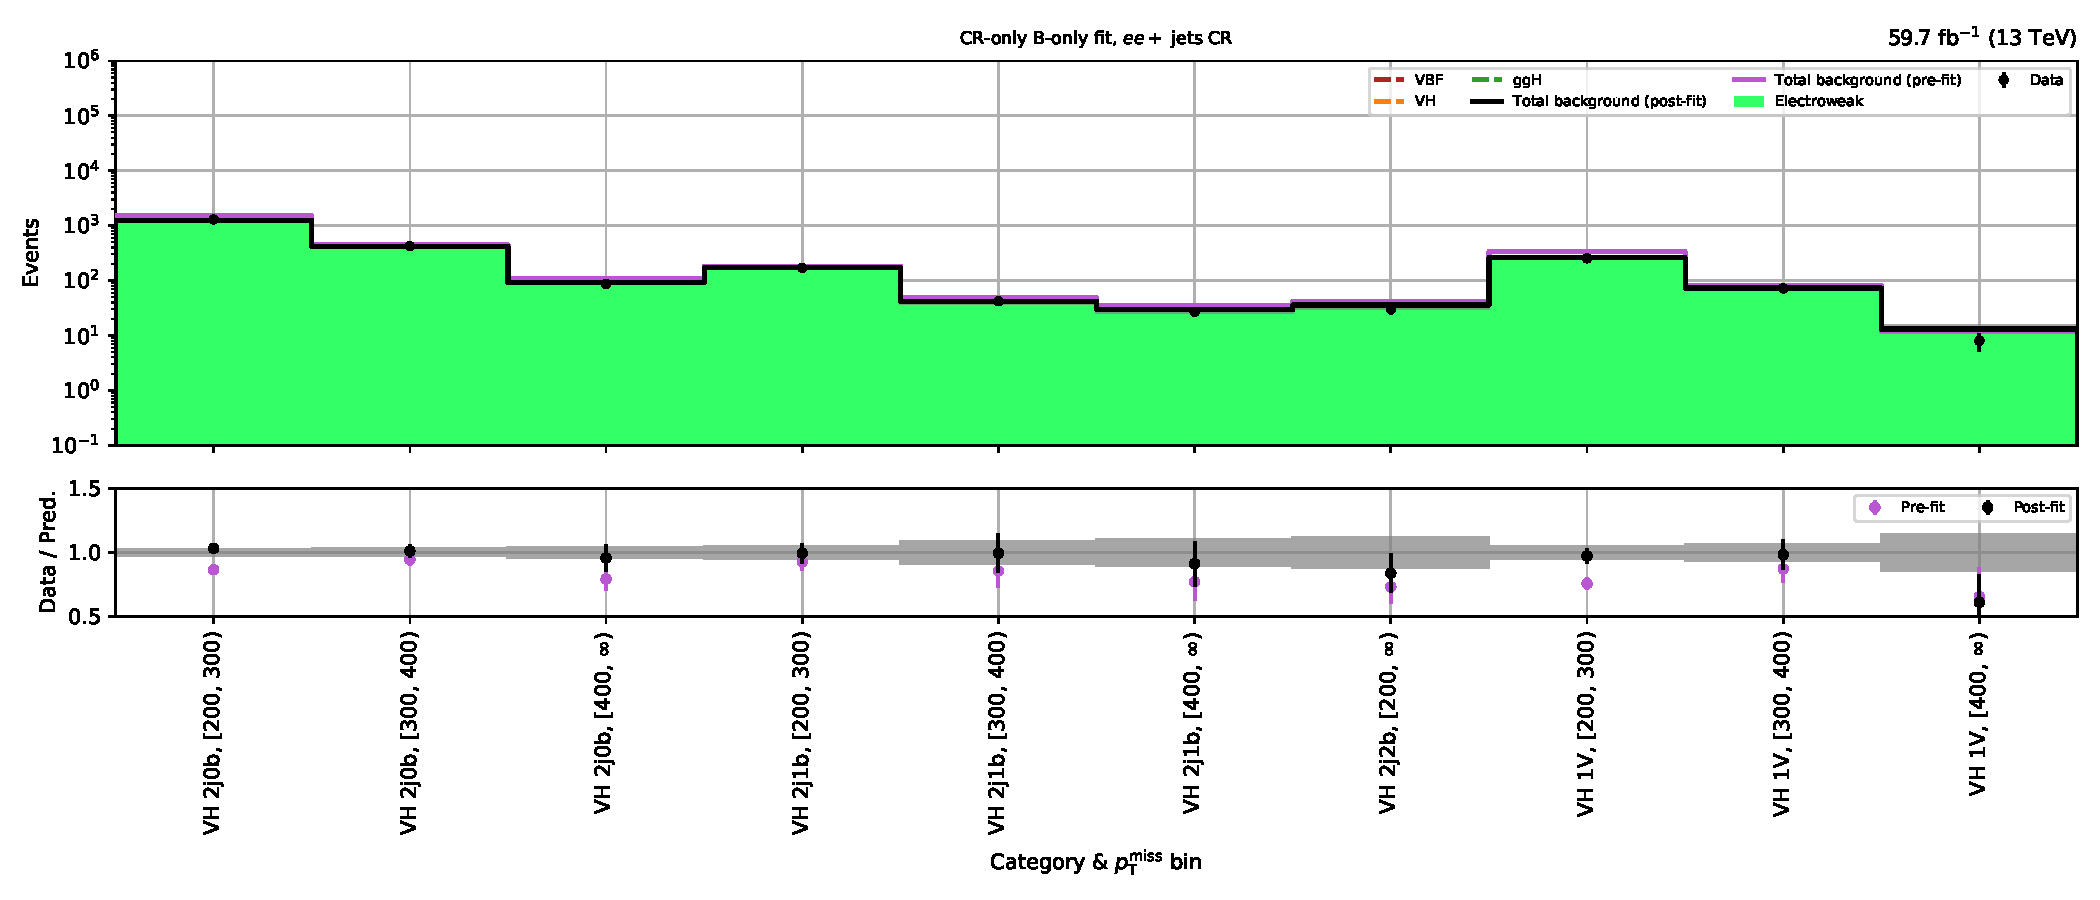
\includegraphics[width=\textwidth]{chapters/higgstoinv/figures/mountain_ranges/2018/VH/Zee_tree_fit_b-abs_values_VH_cats.pdf}
        \caption{\VH --- \doubleEleCr \gls{CR} (2018)}
    \end{subfigure}

    \begin{subfigure}[b]{0.9\textwidth}
        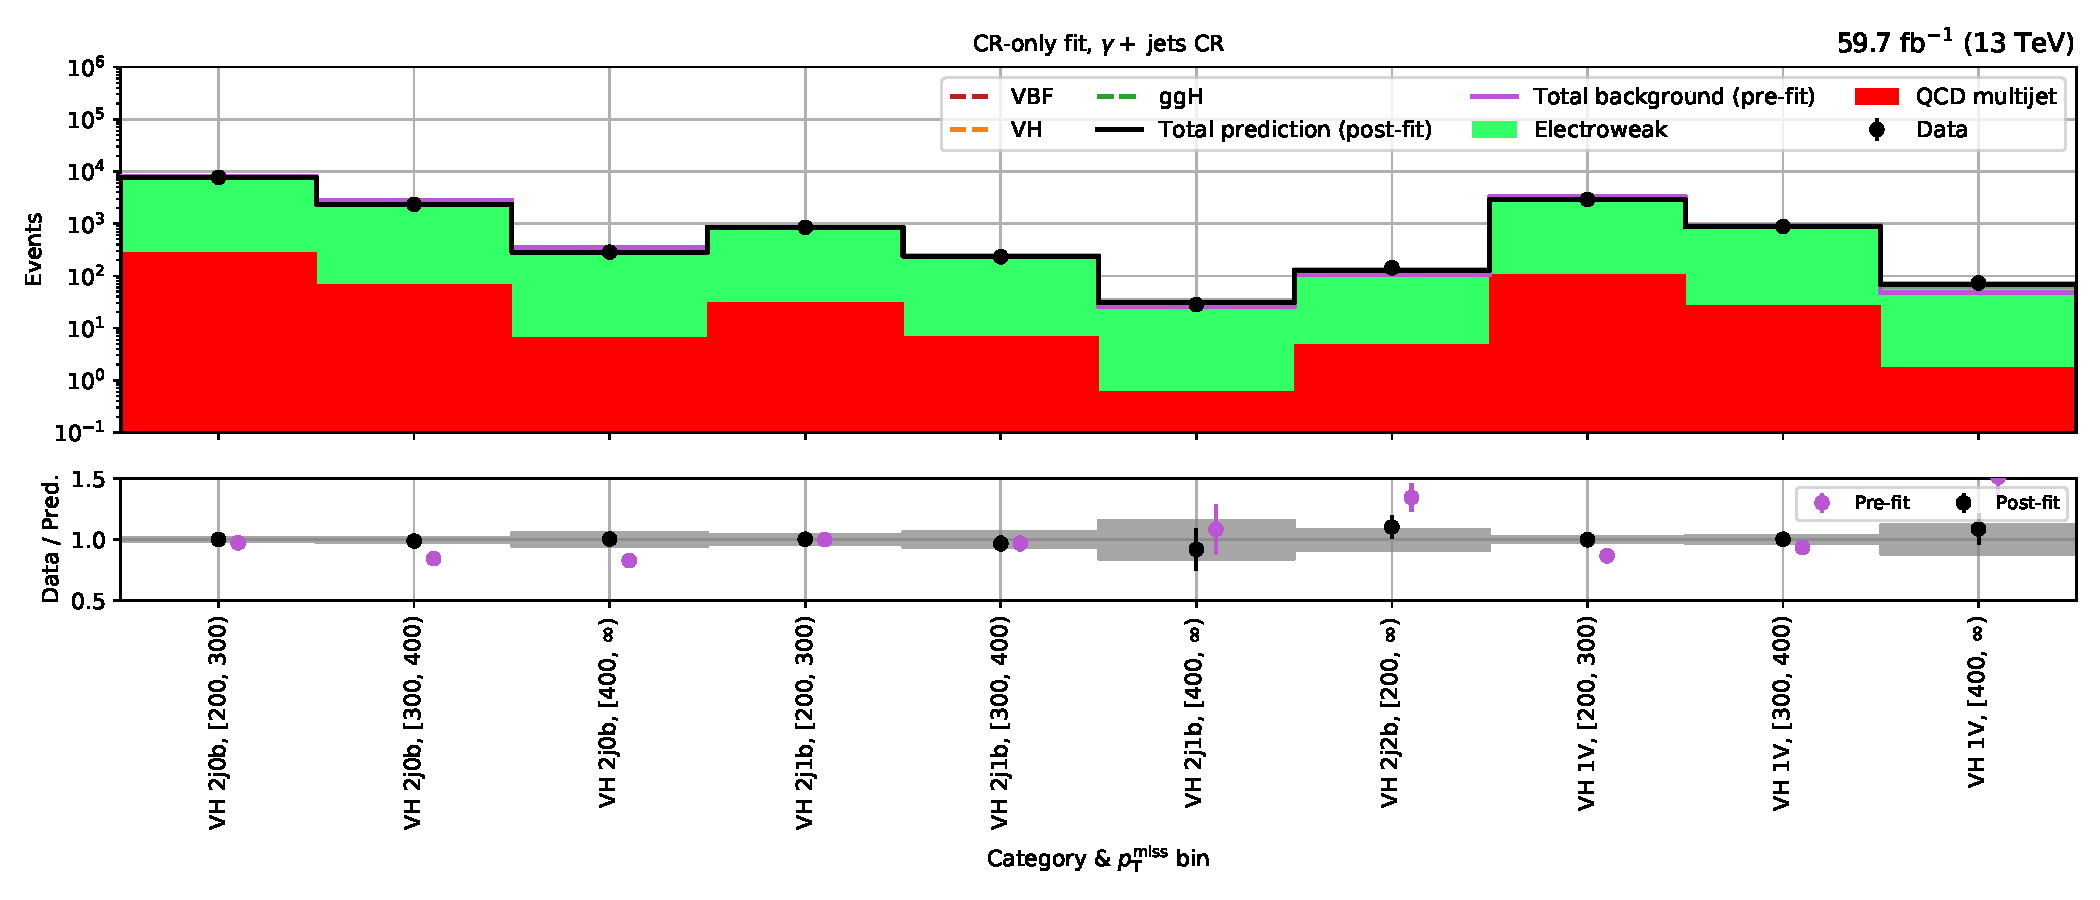
\includegraphics[width=\textwidth]{chapters/higgstoinv/figures/mountain_ranges/2018/VH/Photon_tree_fit_b-abs_values_VH_cats.pdf}
        \caption{\VH --- \singlePhotonCr \gls{CR} (2018)}
    \end{subfigure}
    \caption[Post-fit yields for each \VH category and \ptmiss bin in the dilepton and photon control regions for the 2018 dataset]{Post-fit yields for each \VH category and \ptmiss bin in the dilepton and photon \glspl{CR} for the 2018 dataset. The total background pre-fit and post-fit is compared to data in the lower panel of each subfigure.}
    \label{fig:htoinv_mountain_range_VH_2018_dilep_photon_CRs}
\end{figure}

\clearpage


%=========================================================


\import{./}{rate_params_CR_only_fit.tex}
\clearpage


%=========================================================


\import{./}{qcd_multijet_inputs.tex}
\clearpage


%=========================================================


\section{Background-only fits to the \texorpdfstring{\ttH}{ttH} categories}
\label{sec:B_only_fit_plots_ttH_SR}

\begin{figure}[htbp]
    \centering
    \begin{subfigure}[b]{0.79\textwidth}
        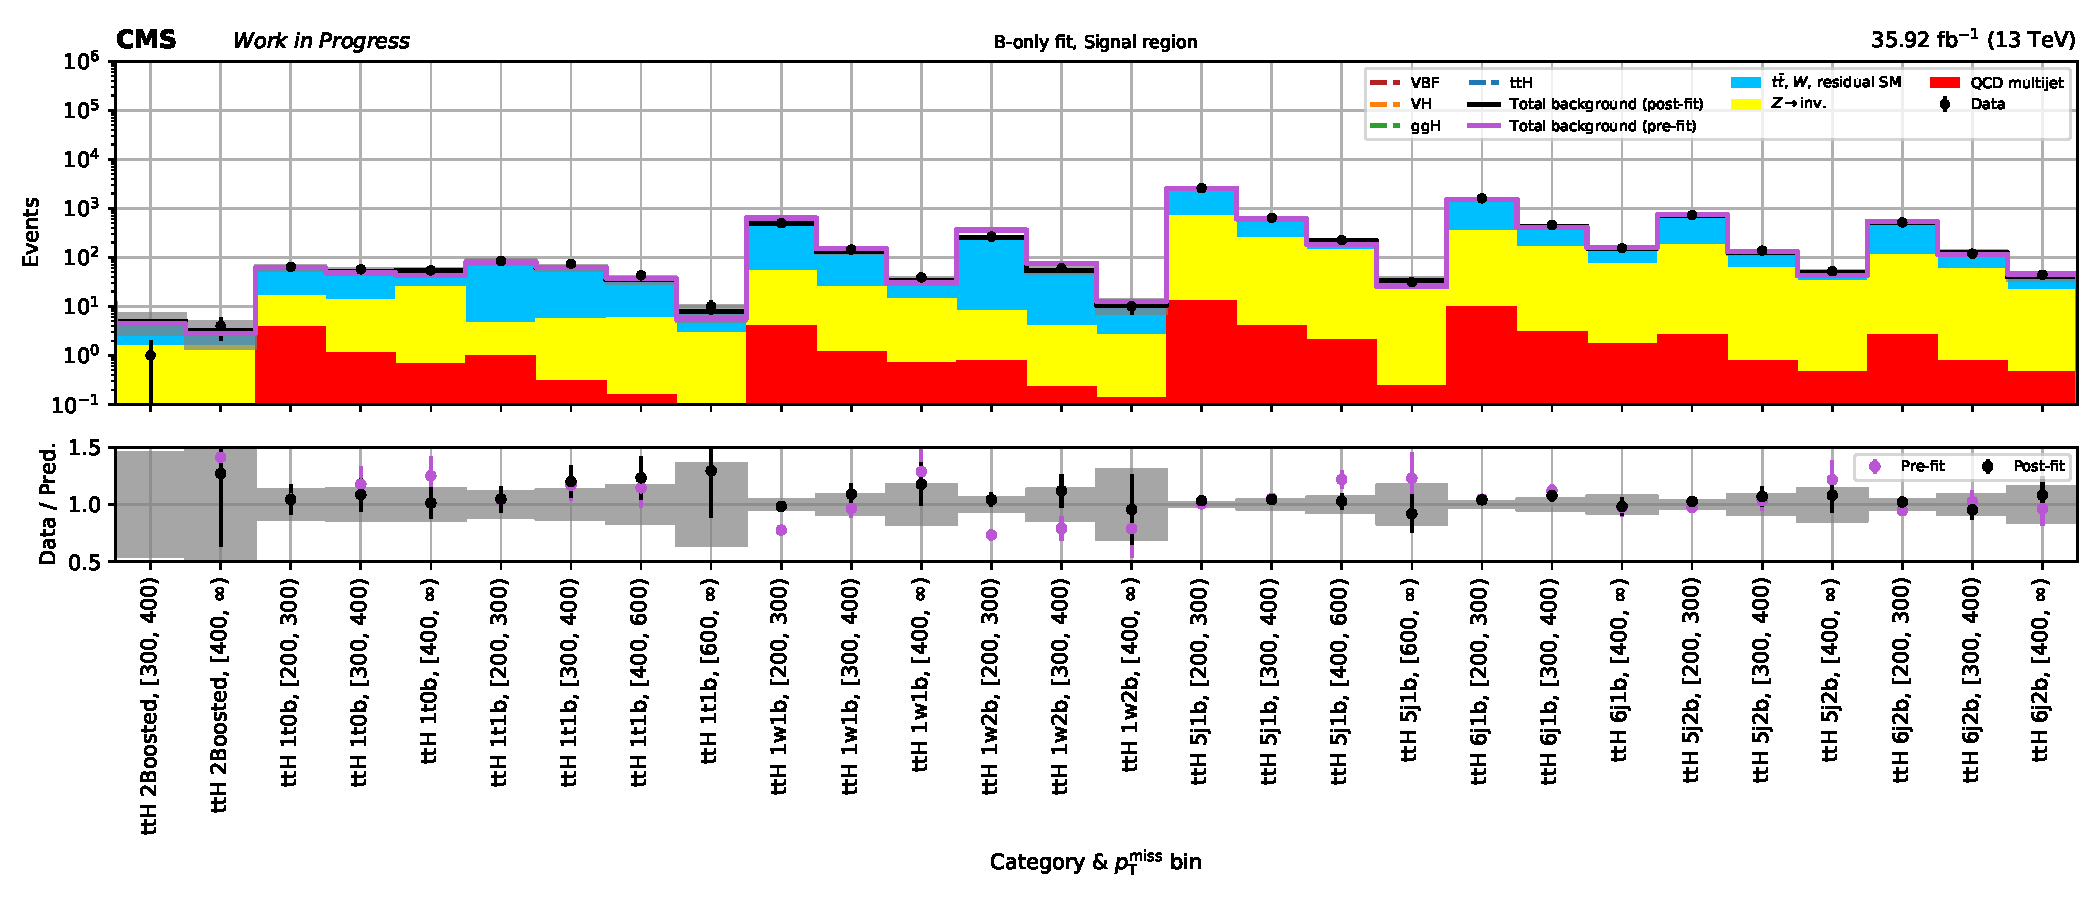
\includegraphics[width=\textwidth]{chapters/higgstoinv/figures/mountain_ranges/2016/ttH/SR_tree_fit_b-abs_values_ttH_cats.pdf}
        \caption{\ttH --- 2016}
    \end{subfigure}

    \begin{subfigure}[b]{0.79\textwidth}
        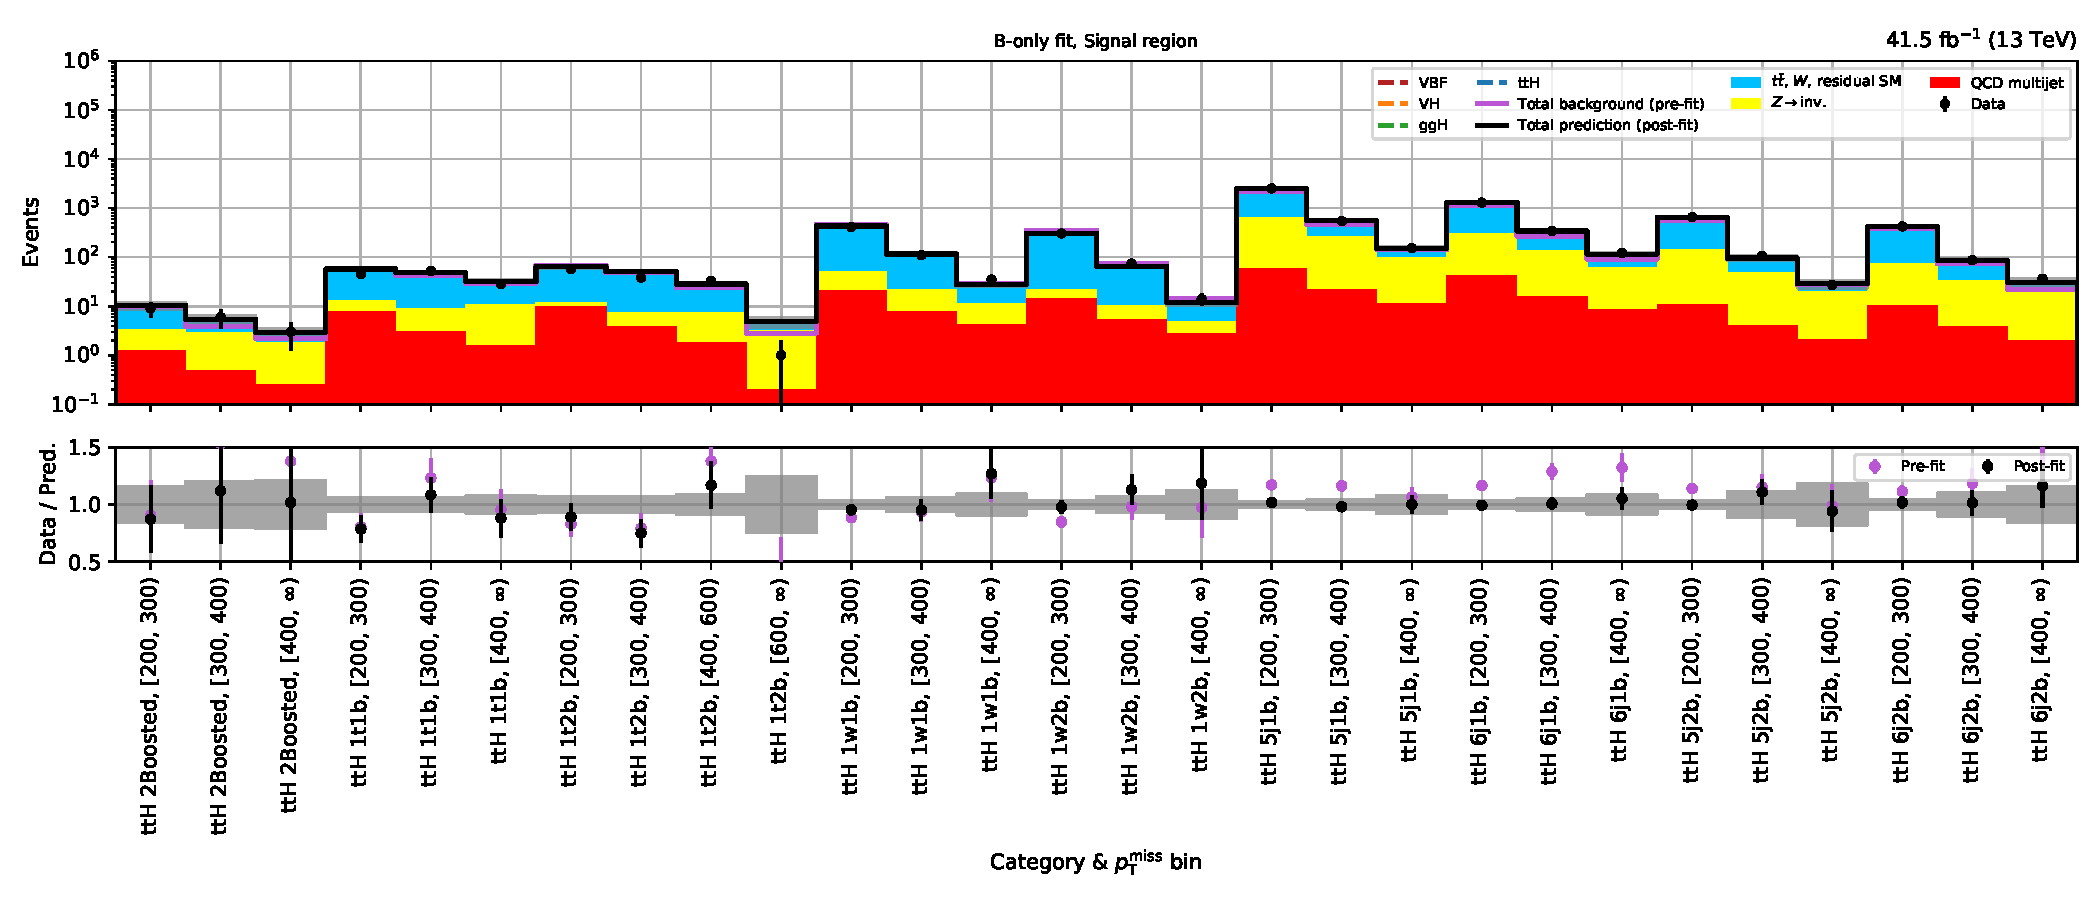
\includegraphics[width=\textwidth]{chapters/higgstoinv/figures/mountain_ranges/2017/ttH/SR_tree_fit_b-abs_values_ttH_cats.pdf}
        \caption{\ttH --- 2017}
    \end{subfigure}

    \begin{subfigure}[b]{0.79\textwidth}
        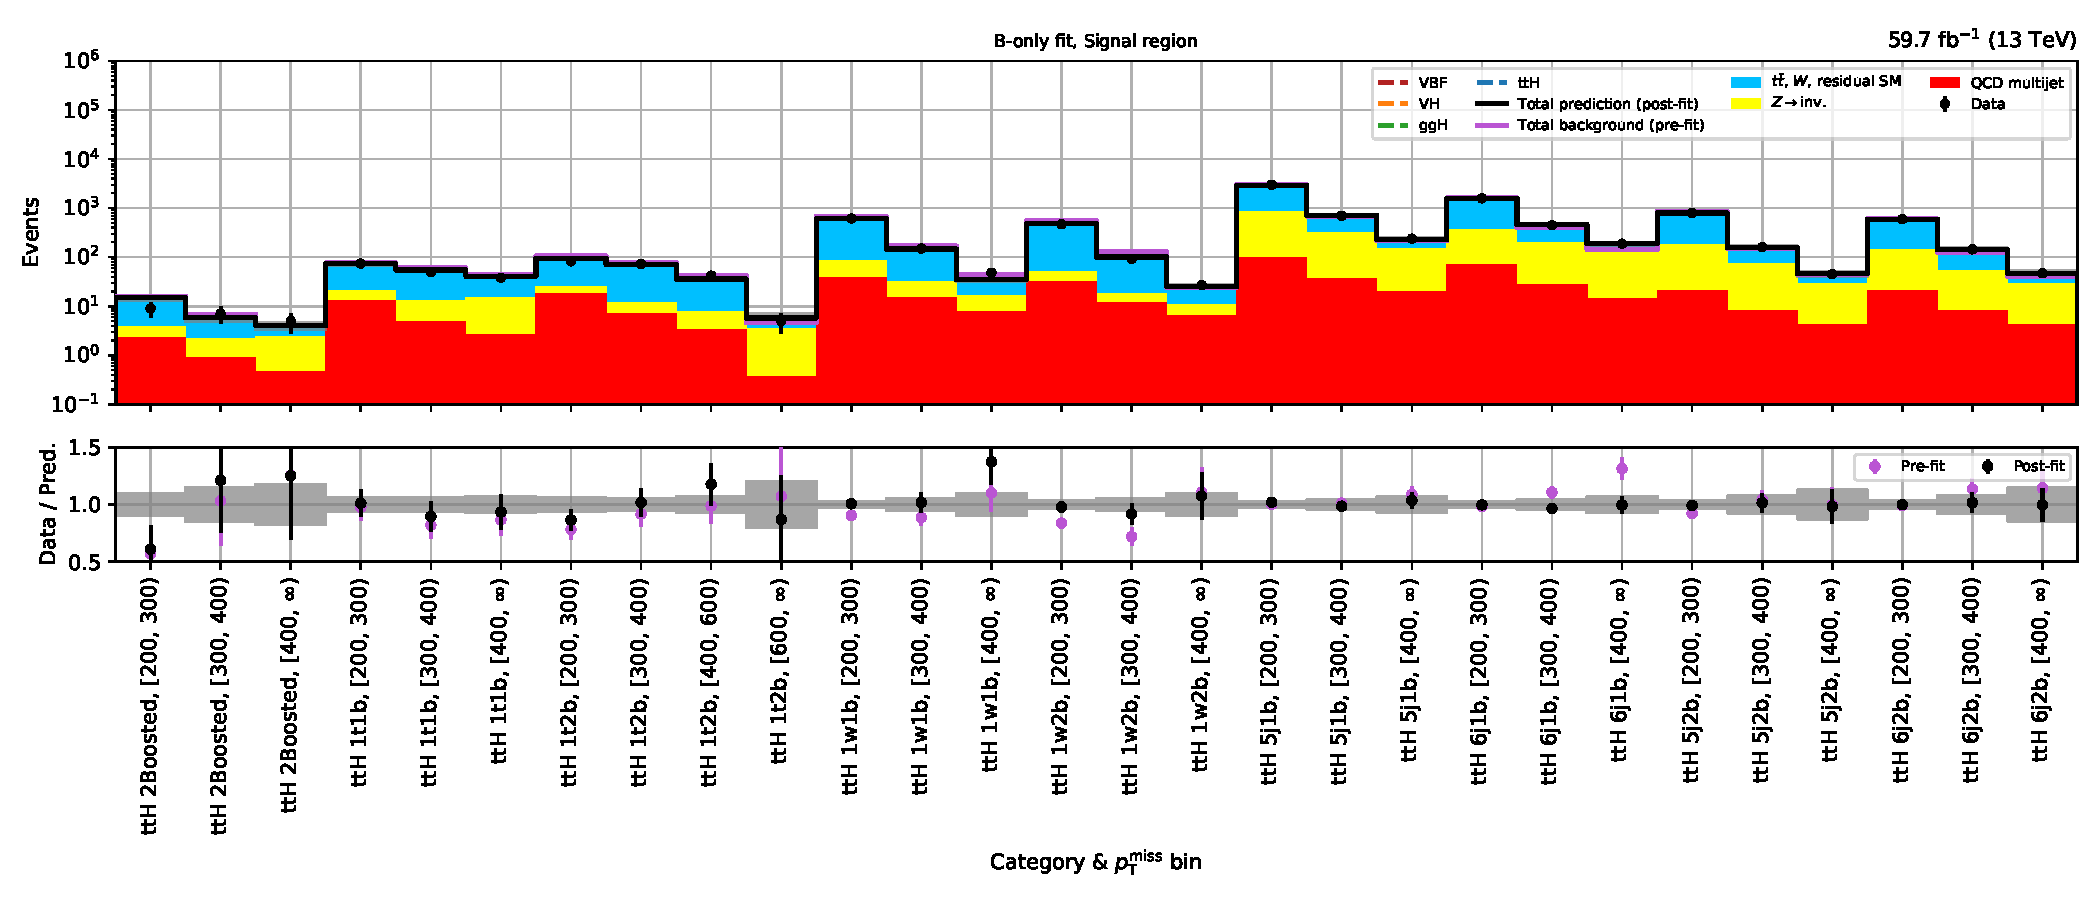
\includegraphics[width=\textwidth]{chapters/higgstoinv/figures/mountain_ranges/2018/ttH/SR_tree_fit_b-abs_values_ttH_cats.pdf}
        \caption{\ttH --- 2018}
    \end{subfigure}
    \caption[Results of the background-only fit to the \ttH categories in each year of Run-2]{Results of the background-only fit to the \ttH categories in each year of Run-2. ``Pre-fit'' refers to outcome of the control region-only prediction.}
    \label{fig:htoinv_mountain_range_B_only_ttH_SR}
\end{figure}

\clearpage


%=========================================================


\section{Background-only fits to the \texorpdfstring{\VH}{VH} categories}
\label{sec:B_only_fit_plots_VH_SR}

\begin{figure}[htbp]
    \centering
    \begin{subfigure}[b]{0.79\textwidth}
        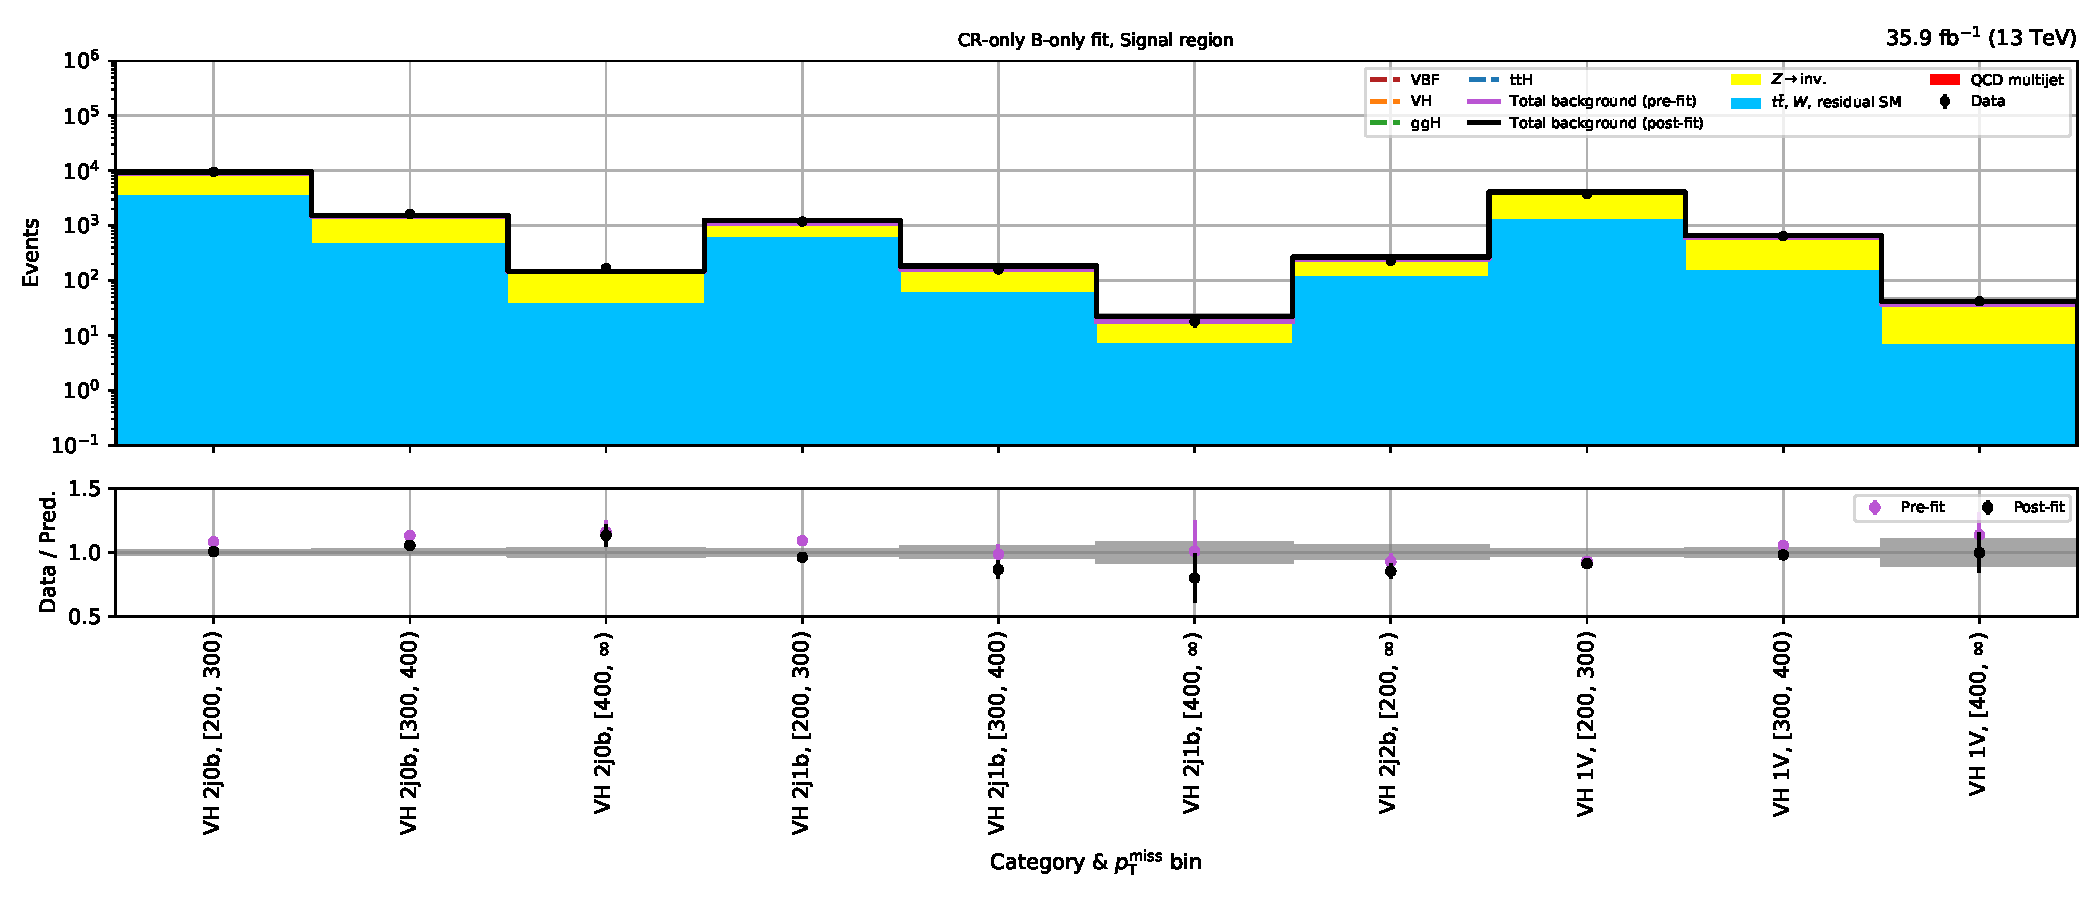
\includegraphics[width=\textwidth]{chapters/higgstoinv/figures/mountain_ranges/2016/VH/SR_tree_fit_b-abs_values_VH_cats.pdf}
        \caption{\VH --- 2016}
    \end{subfigure}

    \begin{subfigure}[b]{0.79\textwidth}
        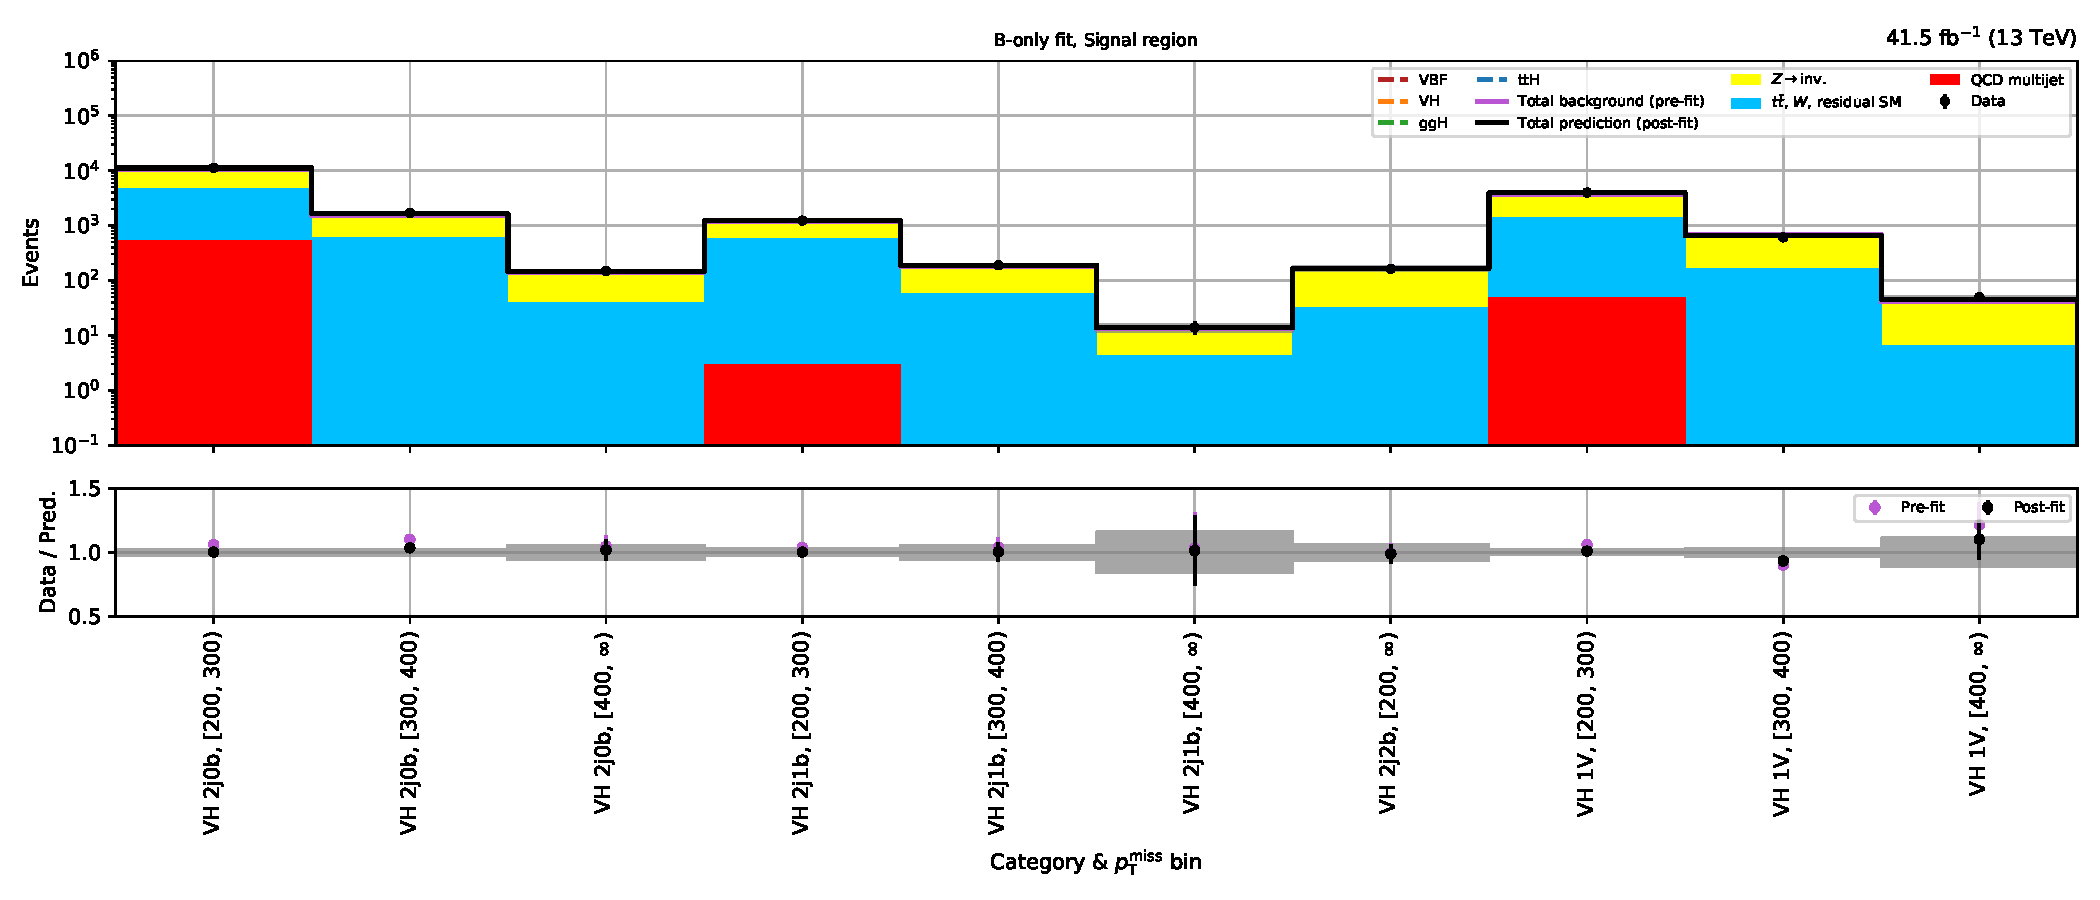
\includegraphics[width=\textwidth]{chapters/higgstoinv/figures/mountain_ranges/2017/VH/SR_tree_fit_b-abs_values_VH_cats.pdf}
        \caption{\VH --- 2017}
    \end{subfigure}

    \begin{subfigure}[b]{0.79\textwidth}
        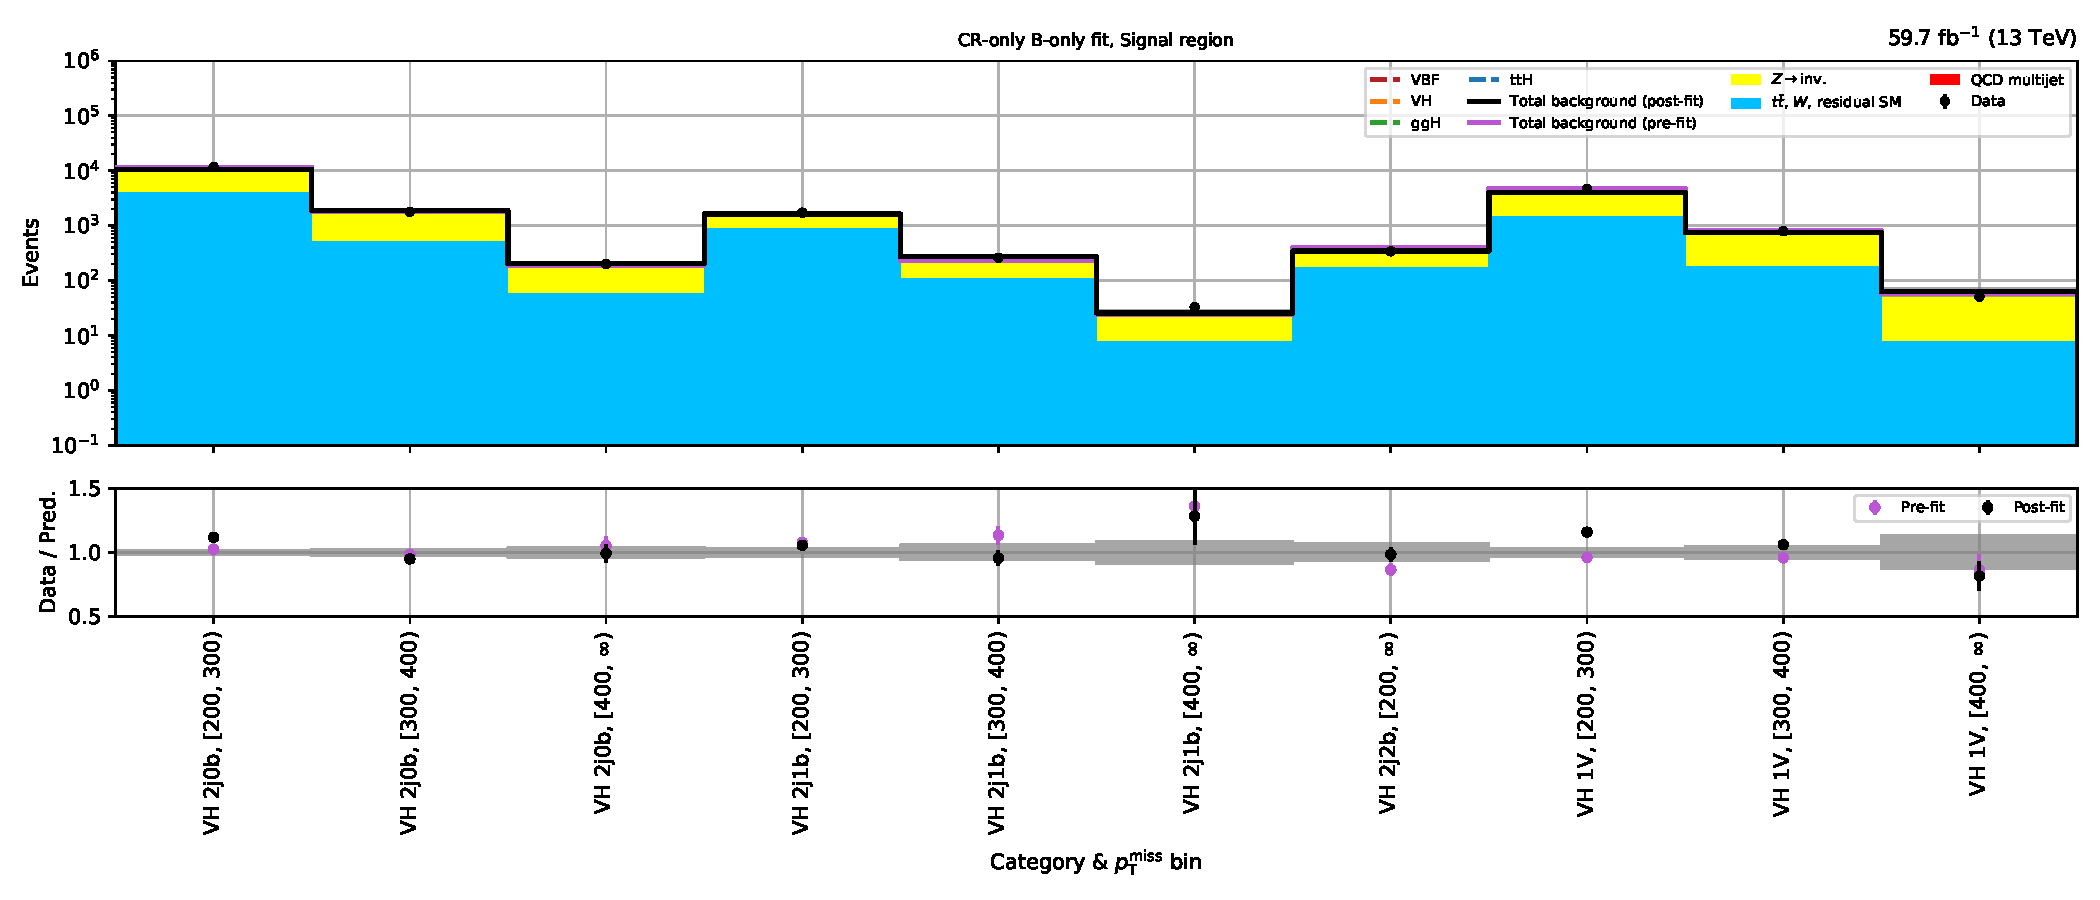
\includegraphics[width=\textwidth]{chapters/higgstoinv/figures/mountain_ranges/2018/VH/SR_tree_fit_b-abs_values_VH_cats.pdf}
        \caption{\VH --- 2018}
    \end{subfigure}
    \caption[Results of the background-only fit to the \VH categories in each year of Run-2]{Results of the background-only fit to the \VH categories in each year of Run-2. ``Pre-fit'' refers to outcome of the control region-only prediction.}
    \label{fig:htoinv_mountain_range_B_only_VH_SR}
\end{figure}

\clearpage


%=========================================================


\section{Limits and likelihood scans for each category}
\label{sec:limits_likelihoods_cats_supplementary}

\begin{figure}[htbp]
    \centering
    \begin{subfigure}[b]{0.49\textwidth}
        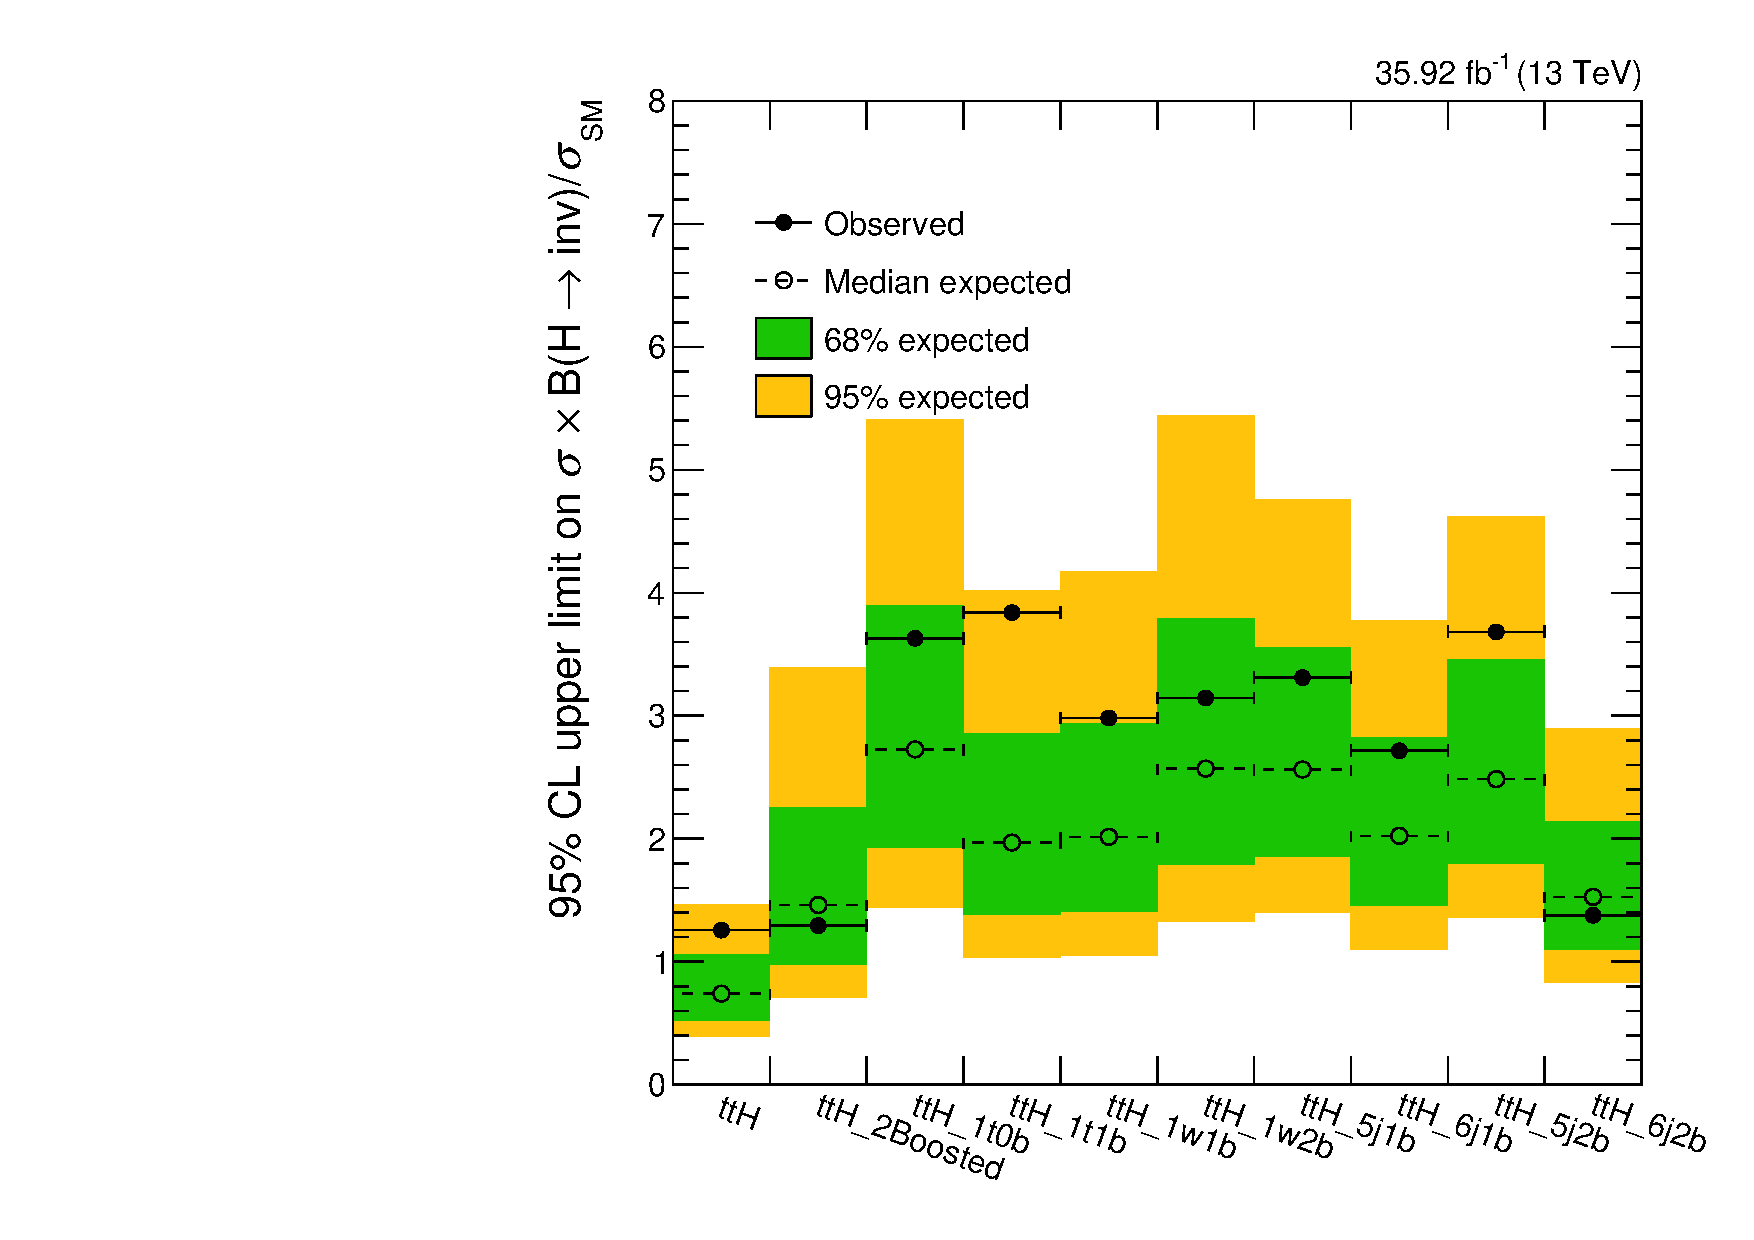
\includegraphics[width=\textwidth]{chapters/higgstoinv/figures/limits/ttH/limit_2016_ttH.pdf}
        \caption{\ttH --- 2016}
    \end{subfigure}
    \hfill
    \begin{subfigure}[b]{0.49\textwidth}
        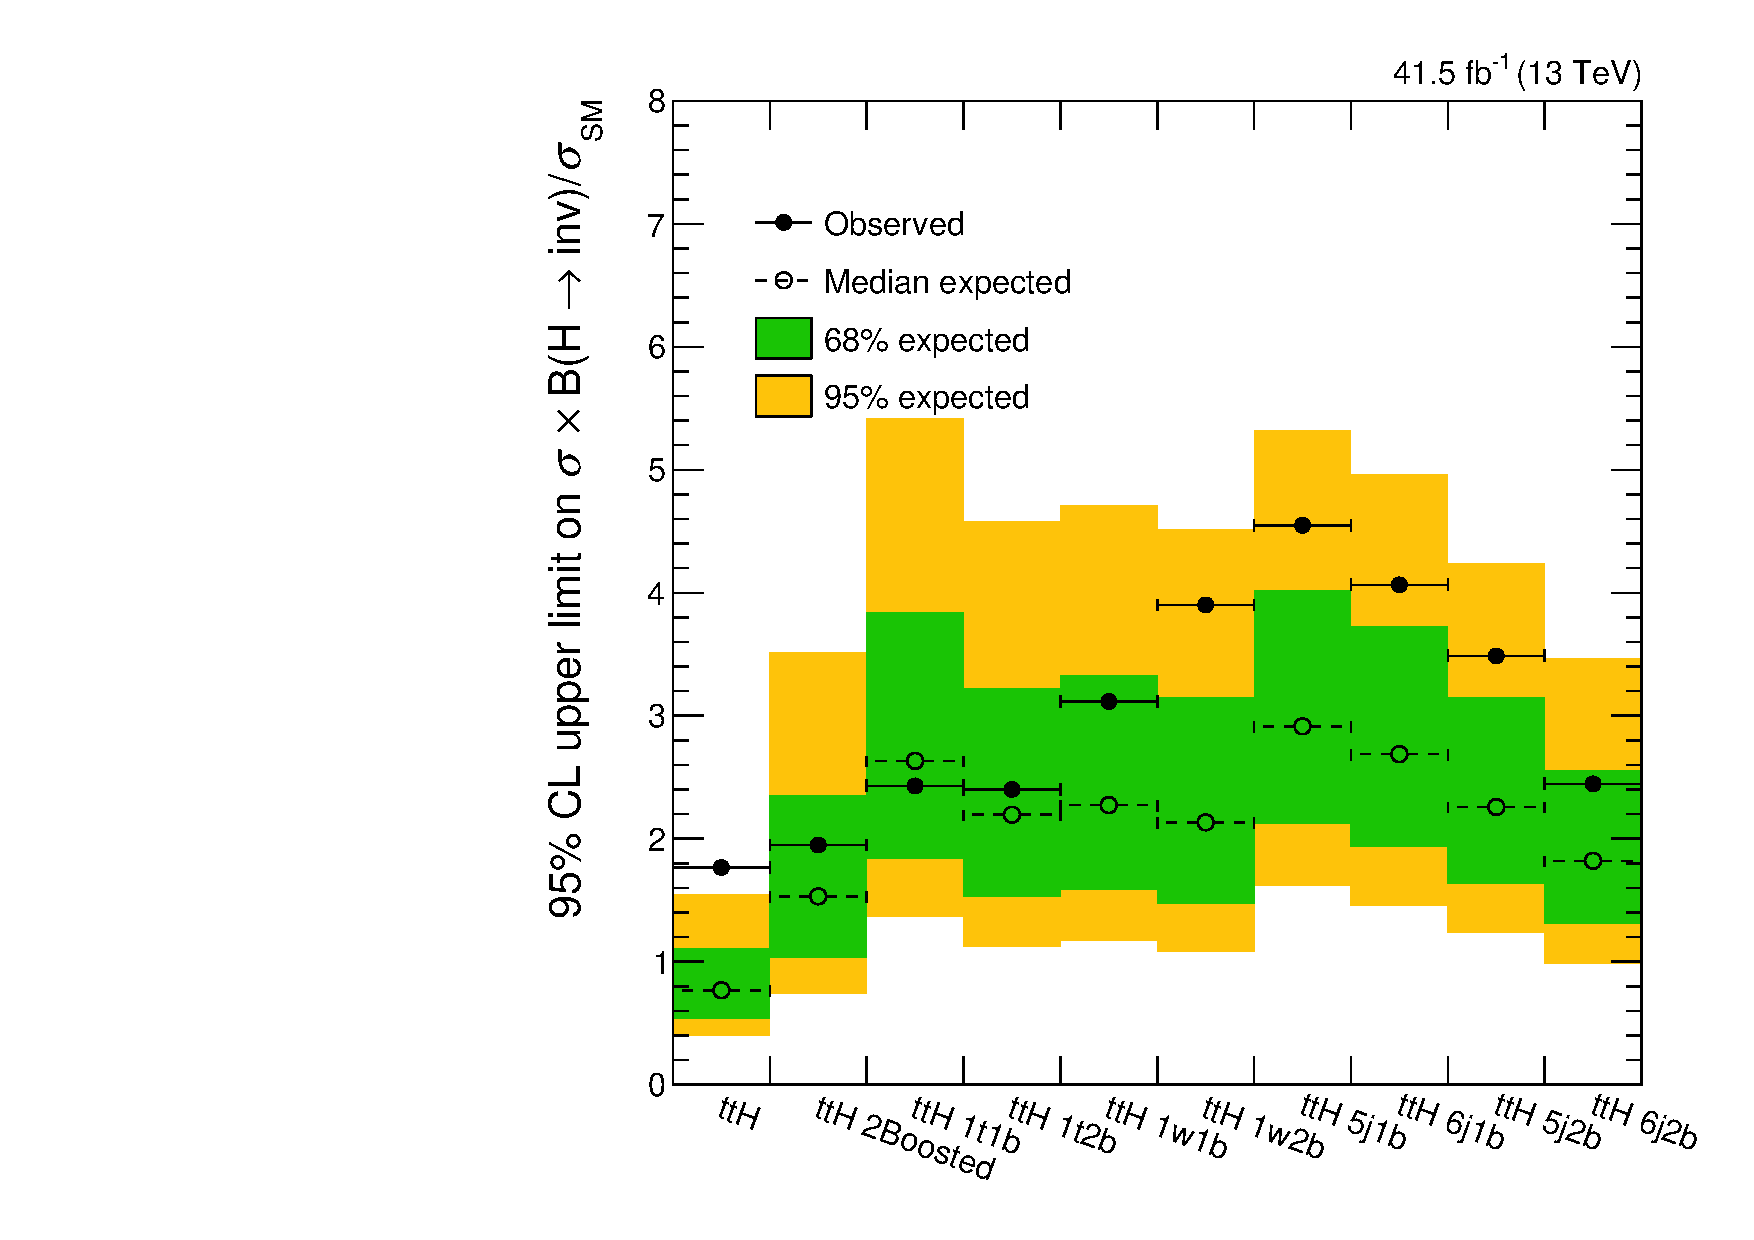
\includegraphics[width=\textwidth]{chapters/higgstoinv/figures/limits/ttH/limit_2017_ttH.pdf}
        \caption{\ttH --- 2017}
    \end{subfigure}

    \begin{subfigure}[b]{0.49\textwidth}
        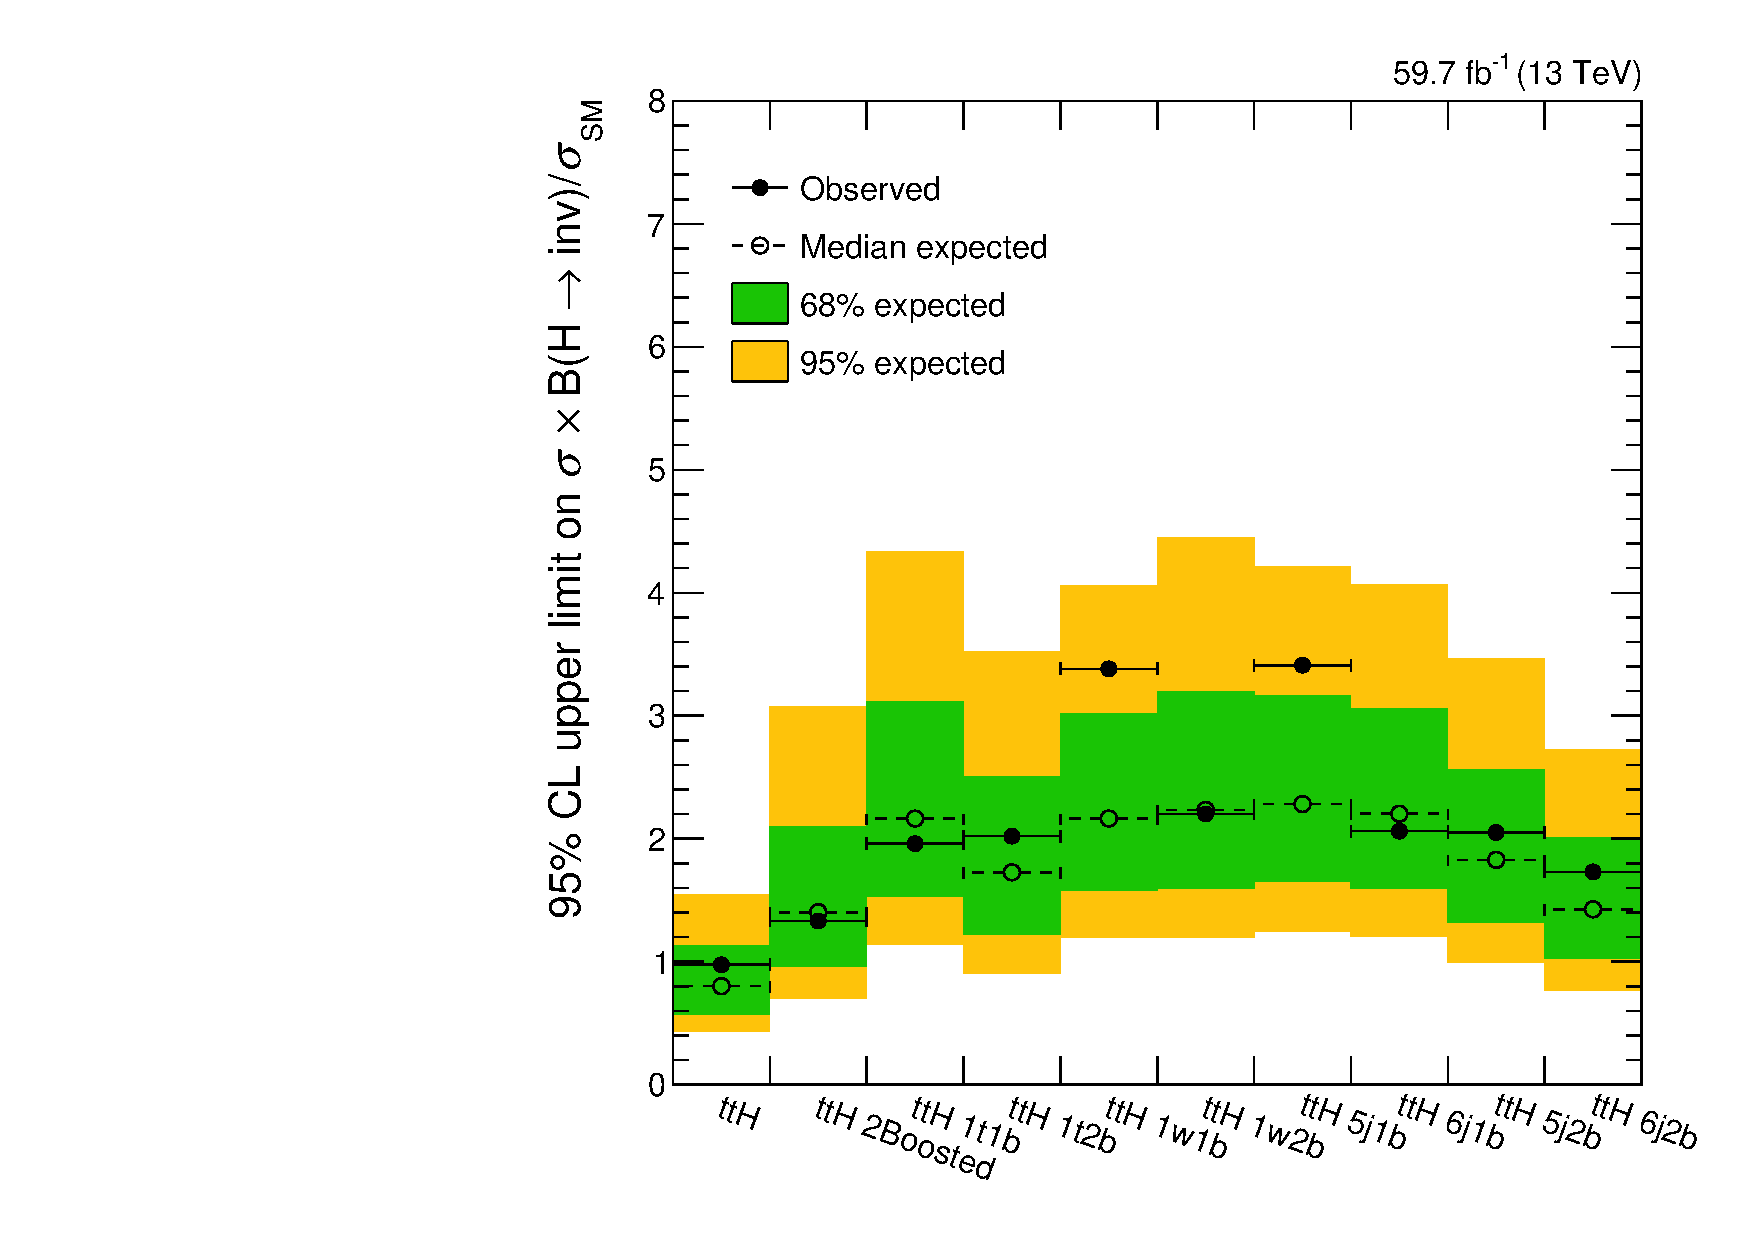
\includegraphics[width=\textwidth]{chapters/higgstoinv/figures/limits/ttH/limit_2018_ttH.pdf}
        \caption{\ttH --- 2018}
    \end{subfigure}
    \caption[Observed and expected 95\,\% CL upper limits on the Higgs boson to invisible state branching fraction in the \ttH channel, for both the individual categories, and the combination of them, for each data-taking year in Run-2]{Observed and expected 95\,\% CL upper limits on the Higgs boson to invisible state branching fraction in the \ttH channel, for both the individual categories, and the combination of them, for each data-taking year in Run-2.}
    \label{fig:htoinv_limit_ttH_per_year}
\end{figure}

\begin{figure}[htbp]
    \centering
    \begin{subfigure}[b]{0.49\textwidth}
        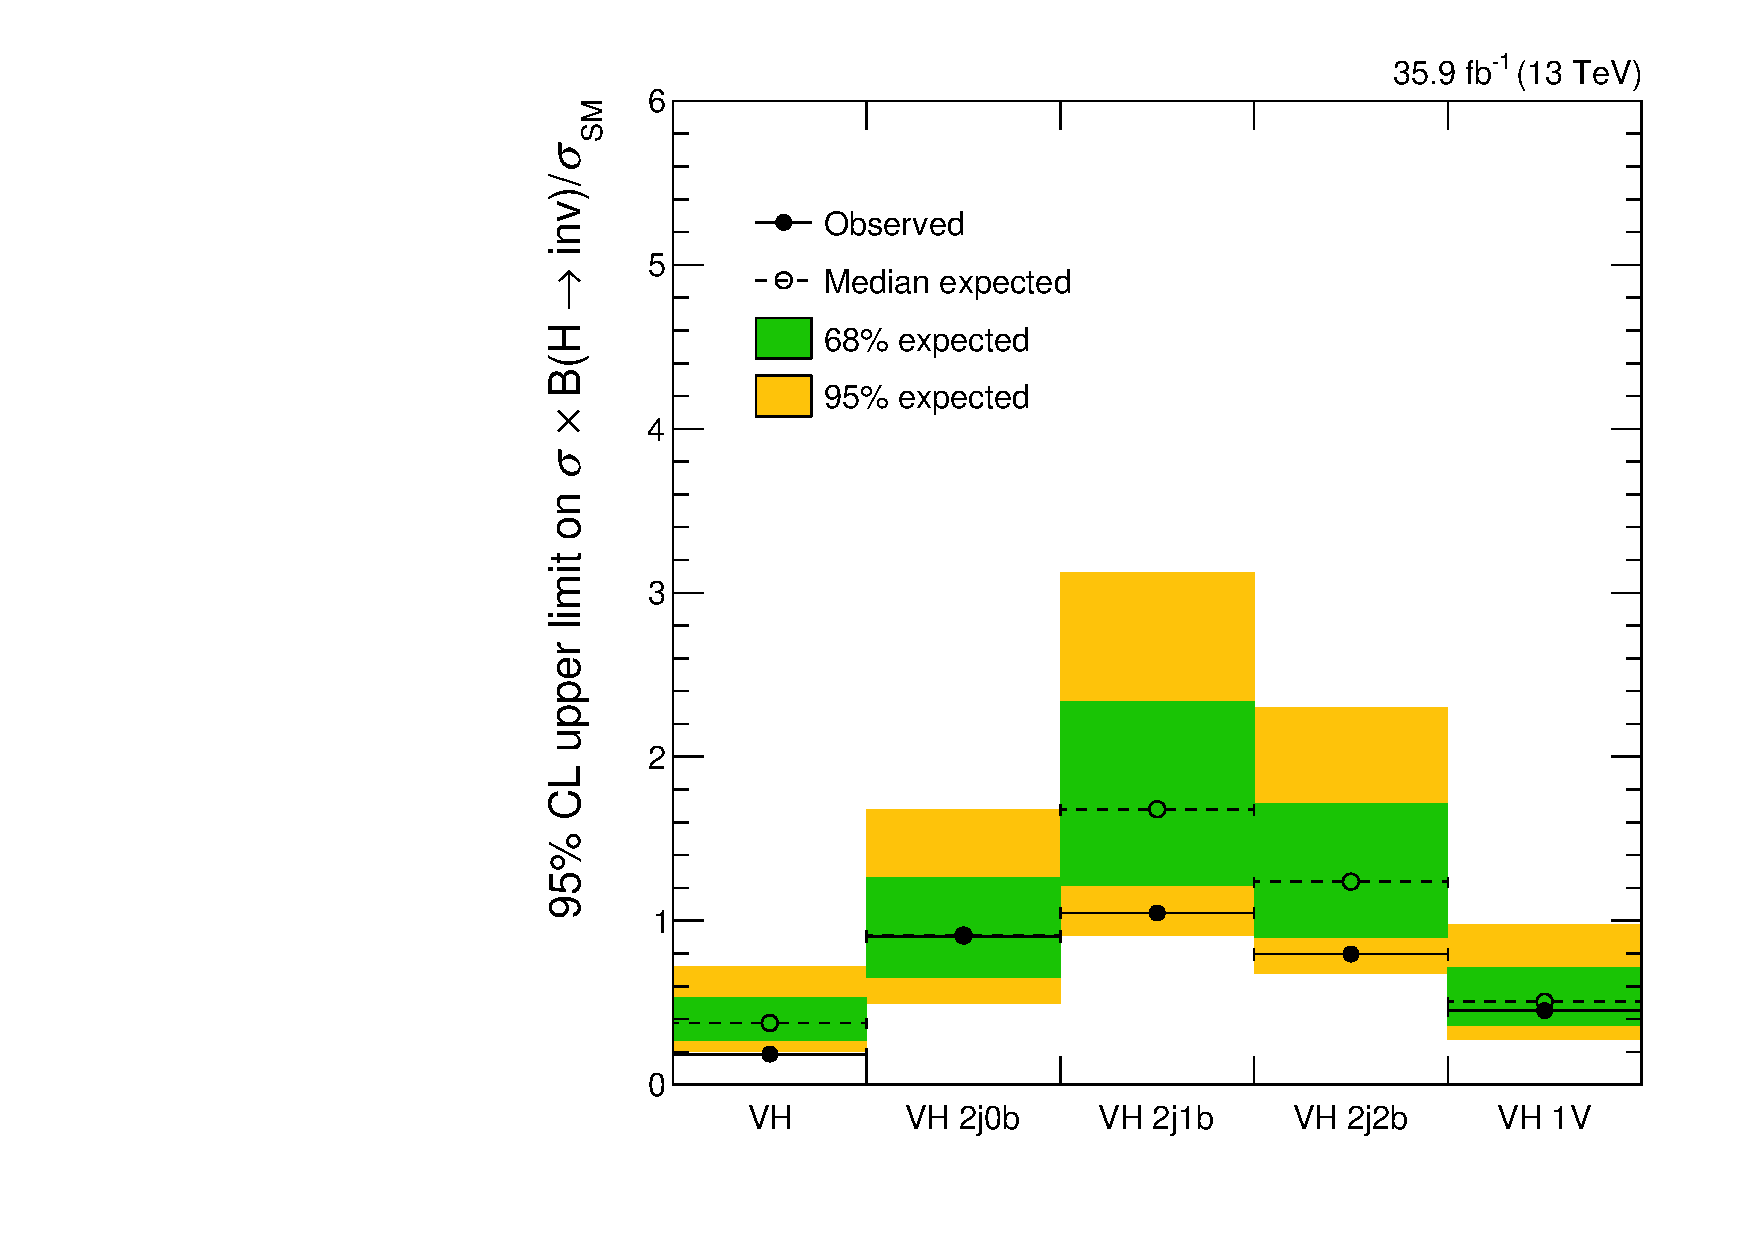
\includegraphics[width=\textwidth]{chapters/higgstoinv/figures/limits/VH/limit_2016_VH.pdf}
        \caption{\VH --- 2016}
        \label{fig:htoinv_limit_VH_2016}
    \end{subfigure}
    \hfill
    \begin{subfigure}[b]{0.49\textwidth}
        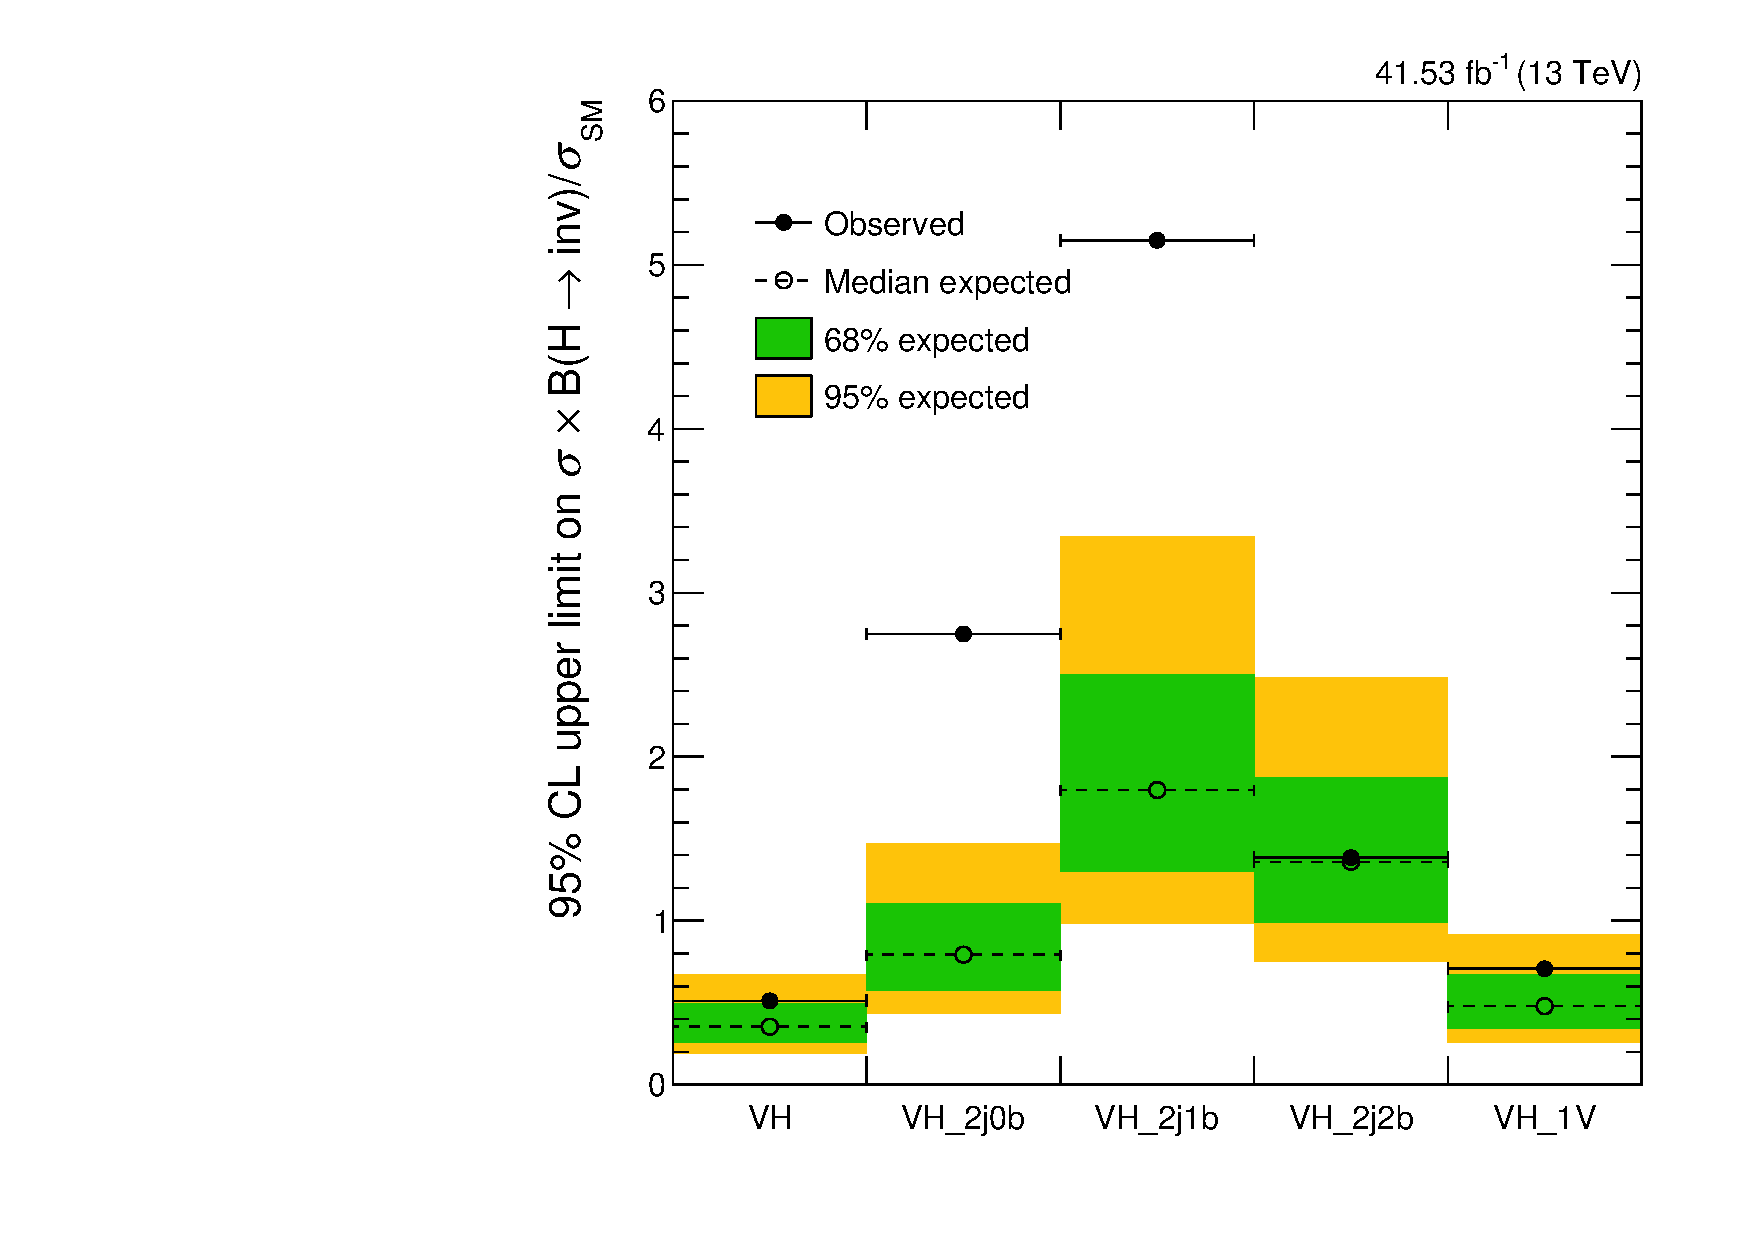
\includegraphics[width=\textwidth]{chapters/higgstoinv/figures/limits/VH/limit_2017_VH.pdf}
        \caption{\VH --- 2017}
    \end{subfigure}

    \begin{subfigure}[b]{0.49\textwidth}
        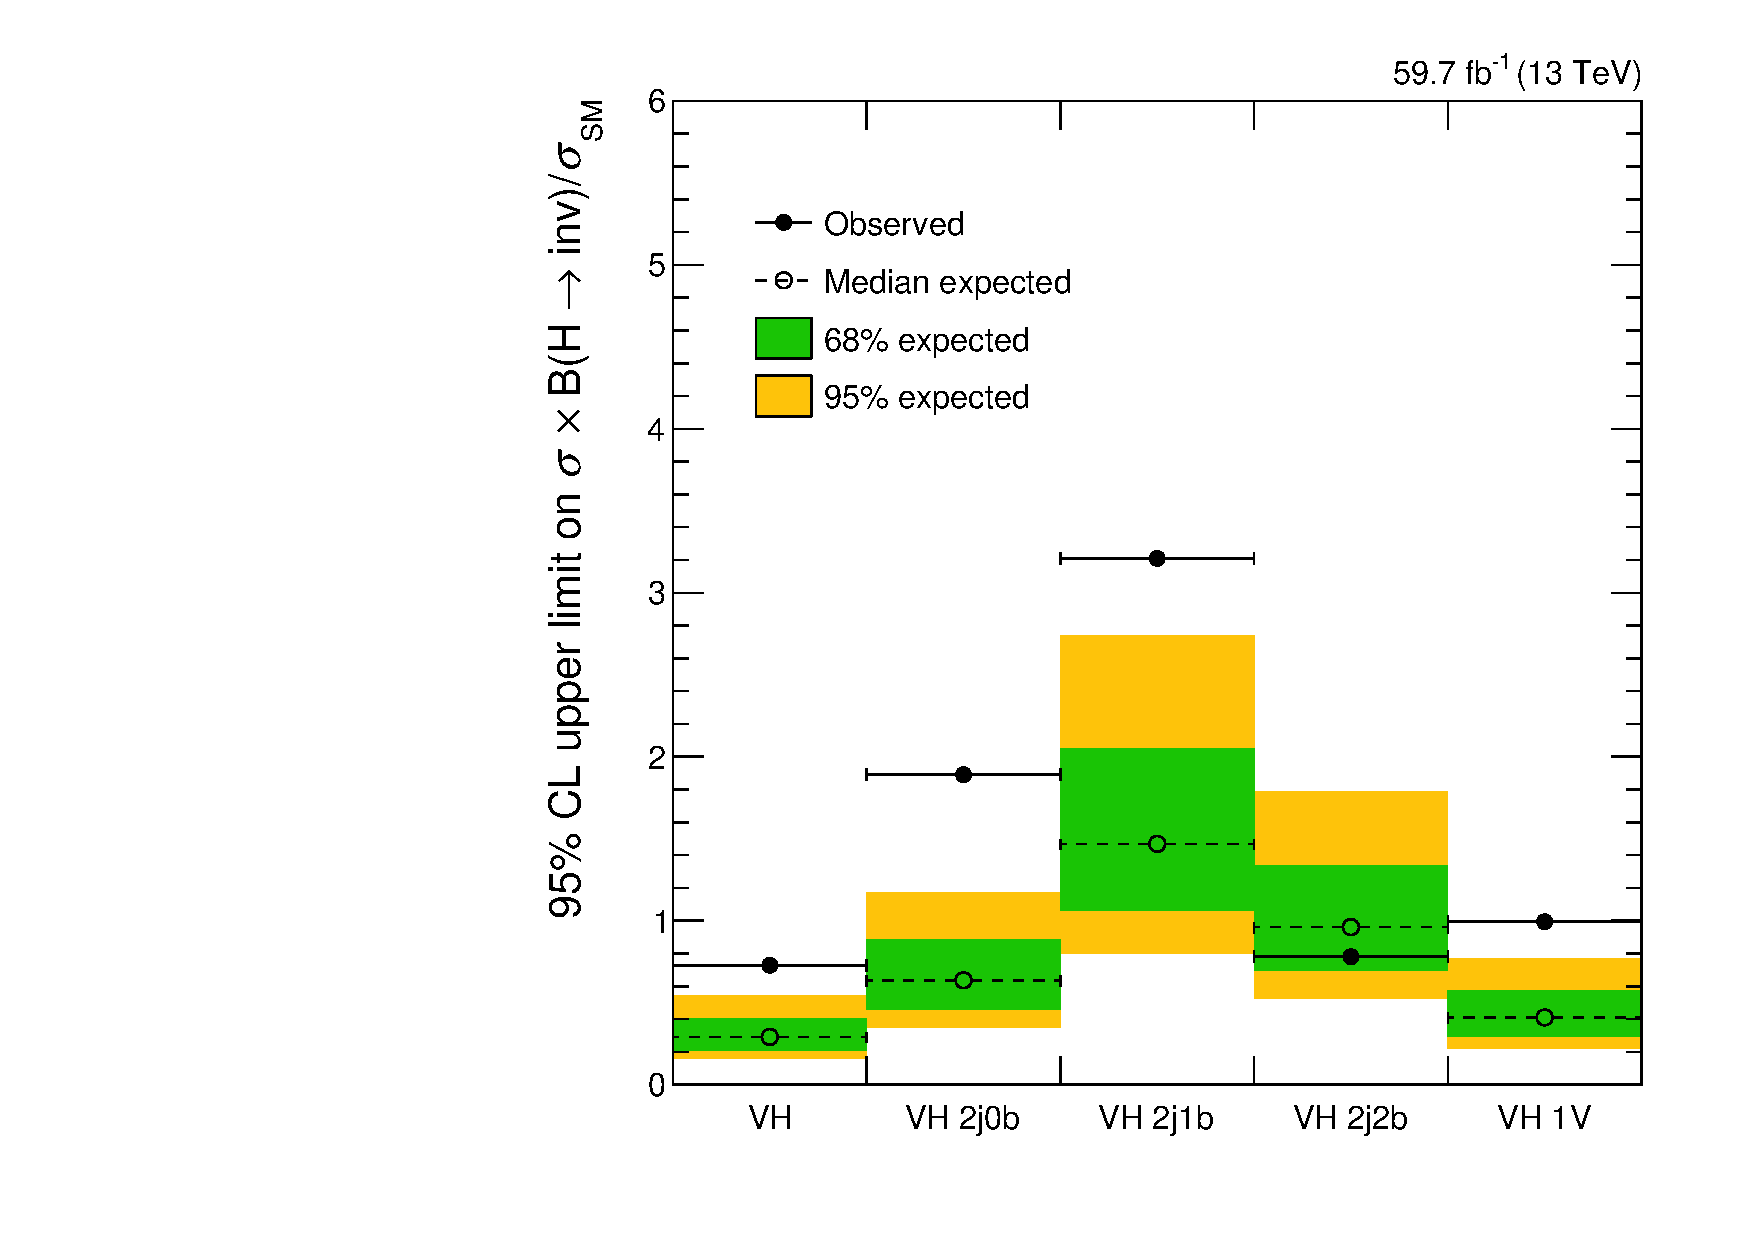
\includegraphics[width=\textwidth]{chapters/higgstoinv/figures/limits/VH/limit_2018_VH.pdf}
        \caption{\VH --- 2018}
    \end{subfigure}
    \caption[Observed and expected 95\,\% CL upper limits on the Higgs boson to invisible state branching fraction in the \VH channel, for both the individual categories, and the combination of them, for each data-taking year in Run-2]{Observed and expected 95\,\% CL upper limits on the Higgs boson to invisible state branching fraction in the \VH channel, for both the individual categories, and the combination of them, for each data-taking year in Run-2.}
    \label{fig:htoinv_limit_VH_per_year}
\end{figure}

\begin{figure}[htbp]
    \centering
    \begin{subfigure}[t]{0.49\textwidth}  % top align since figures are same dimensions, but x-axis labels are larger for likelihood
        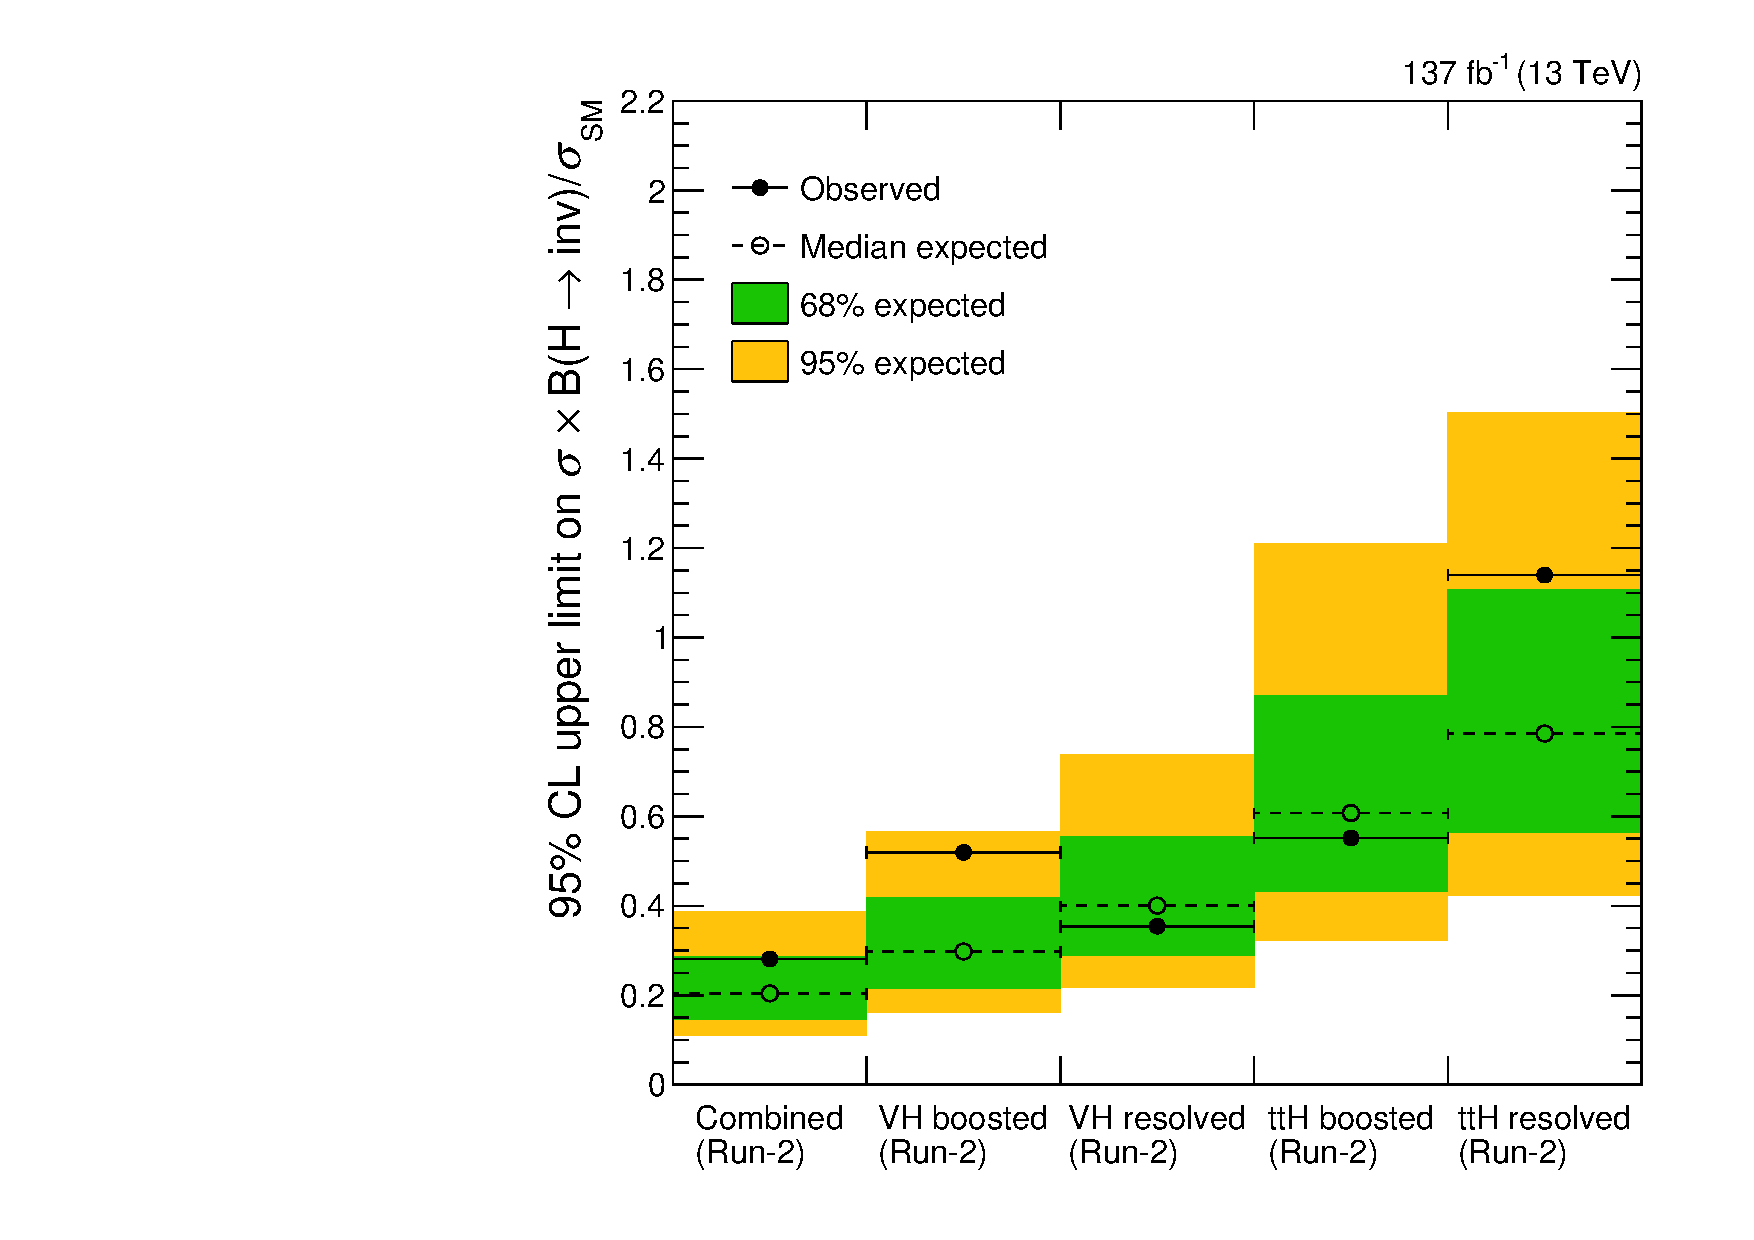
\includegraphics[width=\textwidth]{chapters/higgstoinv/figures/limits/full_Run2/limit_Run2_ttH_VH_resolved_boosted.pdf}
        \caption{Limit --- Run-2}
    \end{subfigure}
    \hfill
    \begin{subfigure}[t]{0.49\textwidth}
        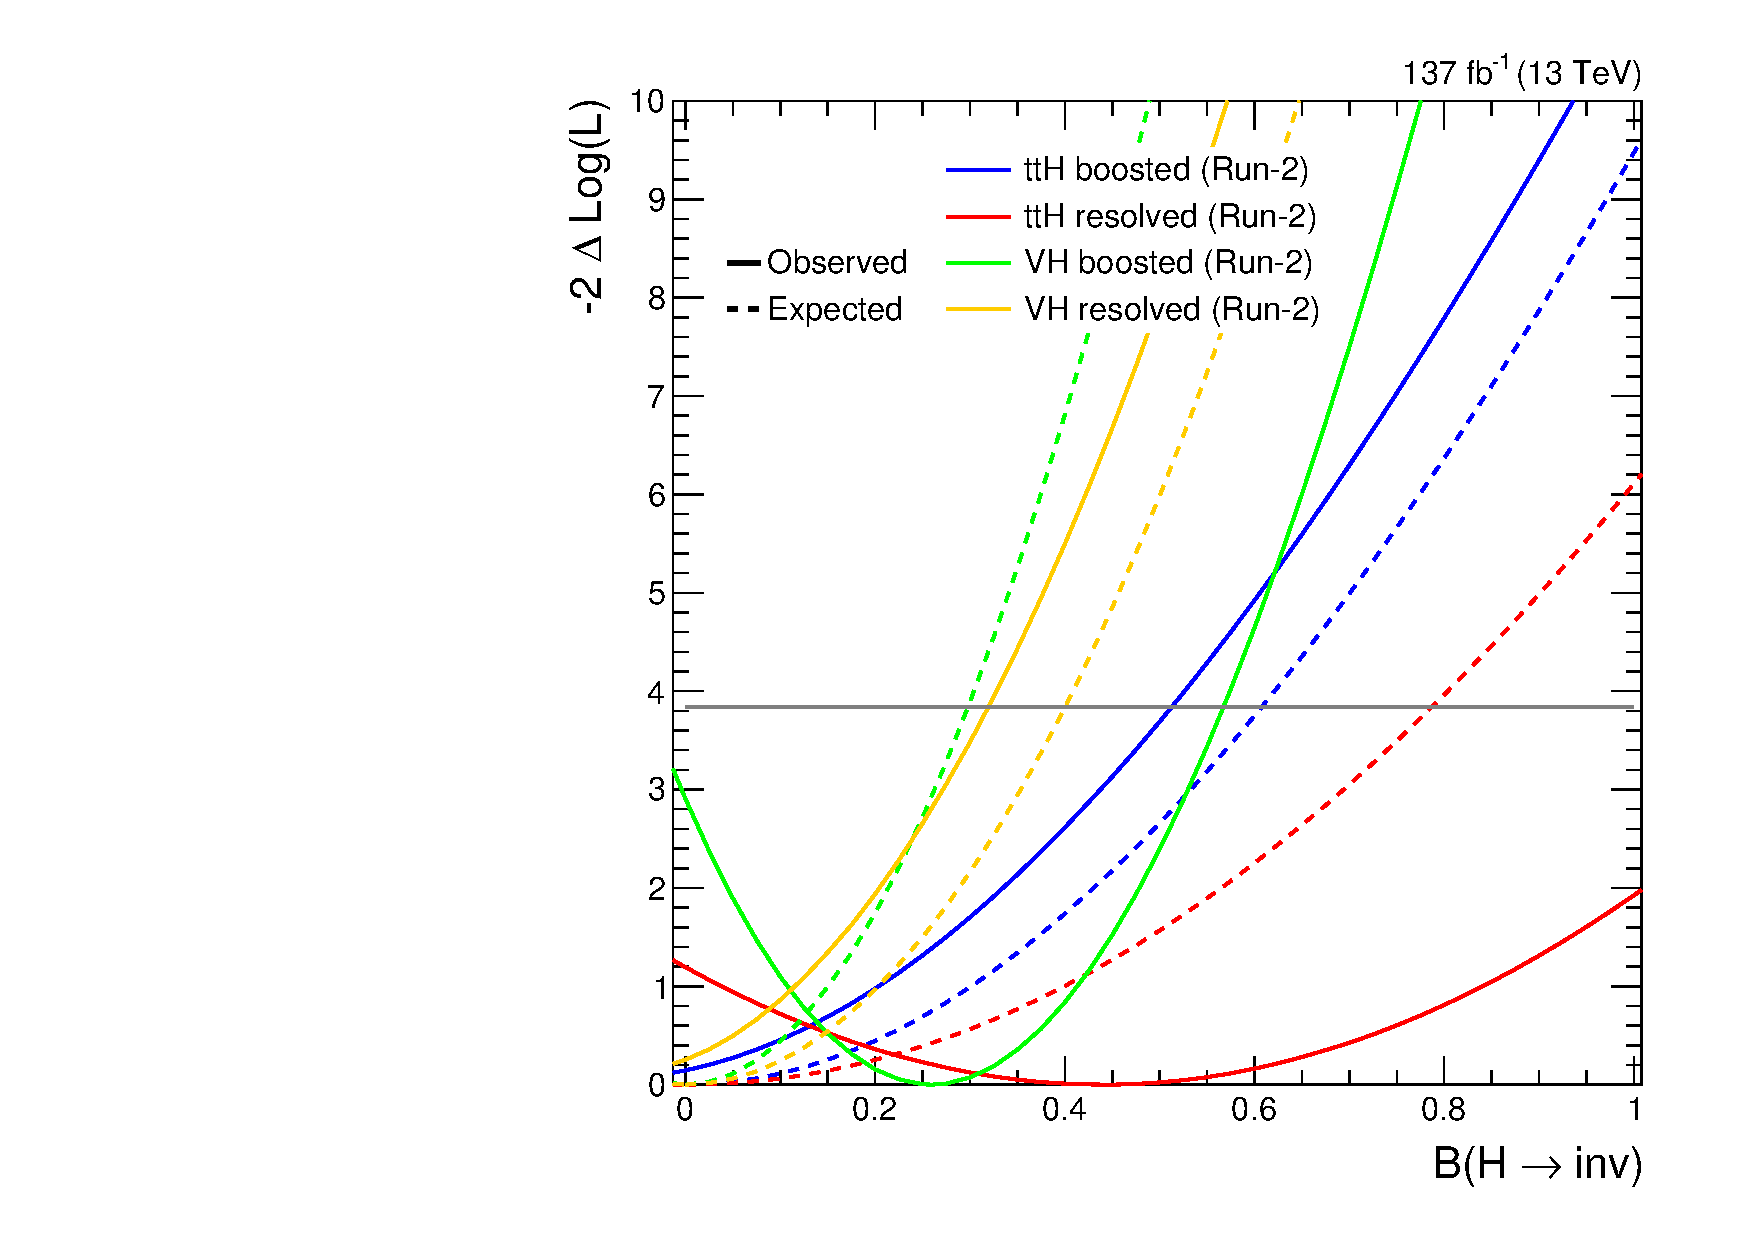
\includegraphics[width=\textwidth]{chapters/higgstoinv/figures/likelihood_scan/profile_likelihood_scan_Run2_ttH_VH_resolved_boosted.pdf}
        \caption{Profile likelihood --- Run-2}
    \end{subfigure}
    \caption[Observed and expected 95\,\% CL upper limit on the Higgs boson to invisible state branching fraction $\BRof{\higgstoinv}$ and the corresponding profile likelihood scan, in the \ttH and \VH boosted and resolved category groupings and their combination, for the full Run-2 dataset]{Observed and expected 95\,\% CL upper limit on the Higgs boson to invisible state branching fraction $\BRof{\higgstoinv}$ (left) and the corresponding profile likelihood scan (right), in the \ttH and \VH boosted and resolved category groupings and their combination, for the full Run-2 dataset.}
    \label{fig:htoinv_limit_likelihood_boosted_resolved_cats_Run2}
\end{figure}
